%!TEX root = main.tex
\clearpage
% fig:stableness_rp
% The rank percentile indicators are stable over publishing years 
\begin{figure}[ht!]
    \centering
    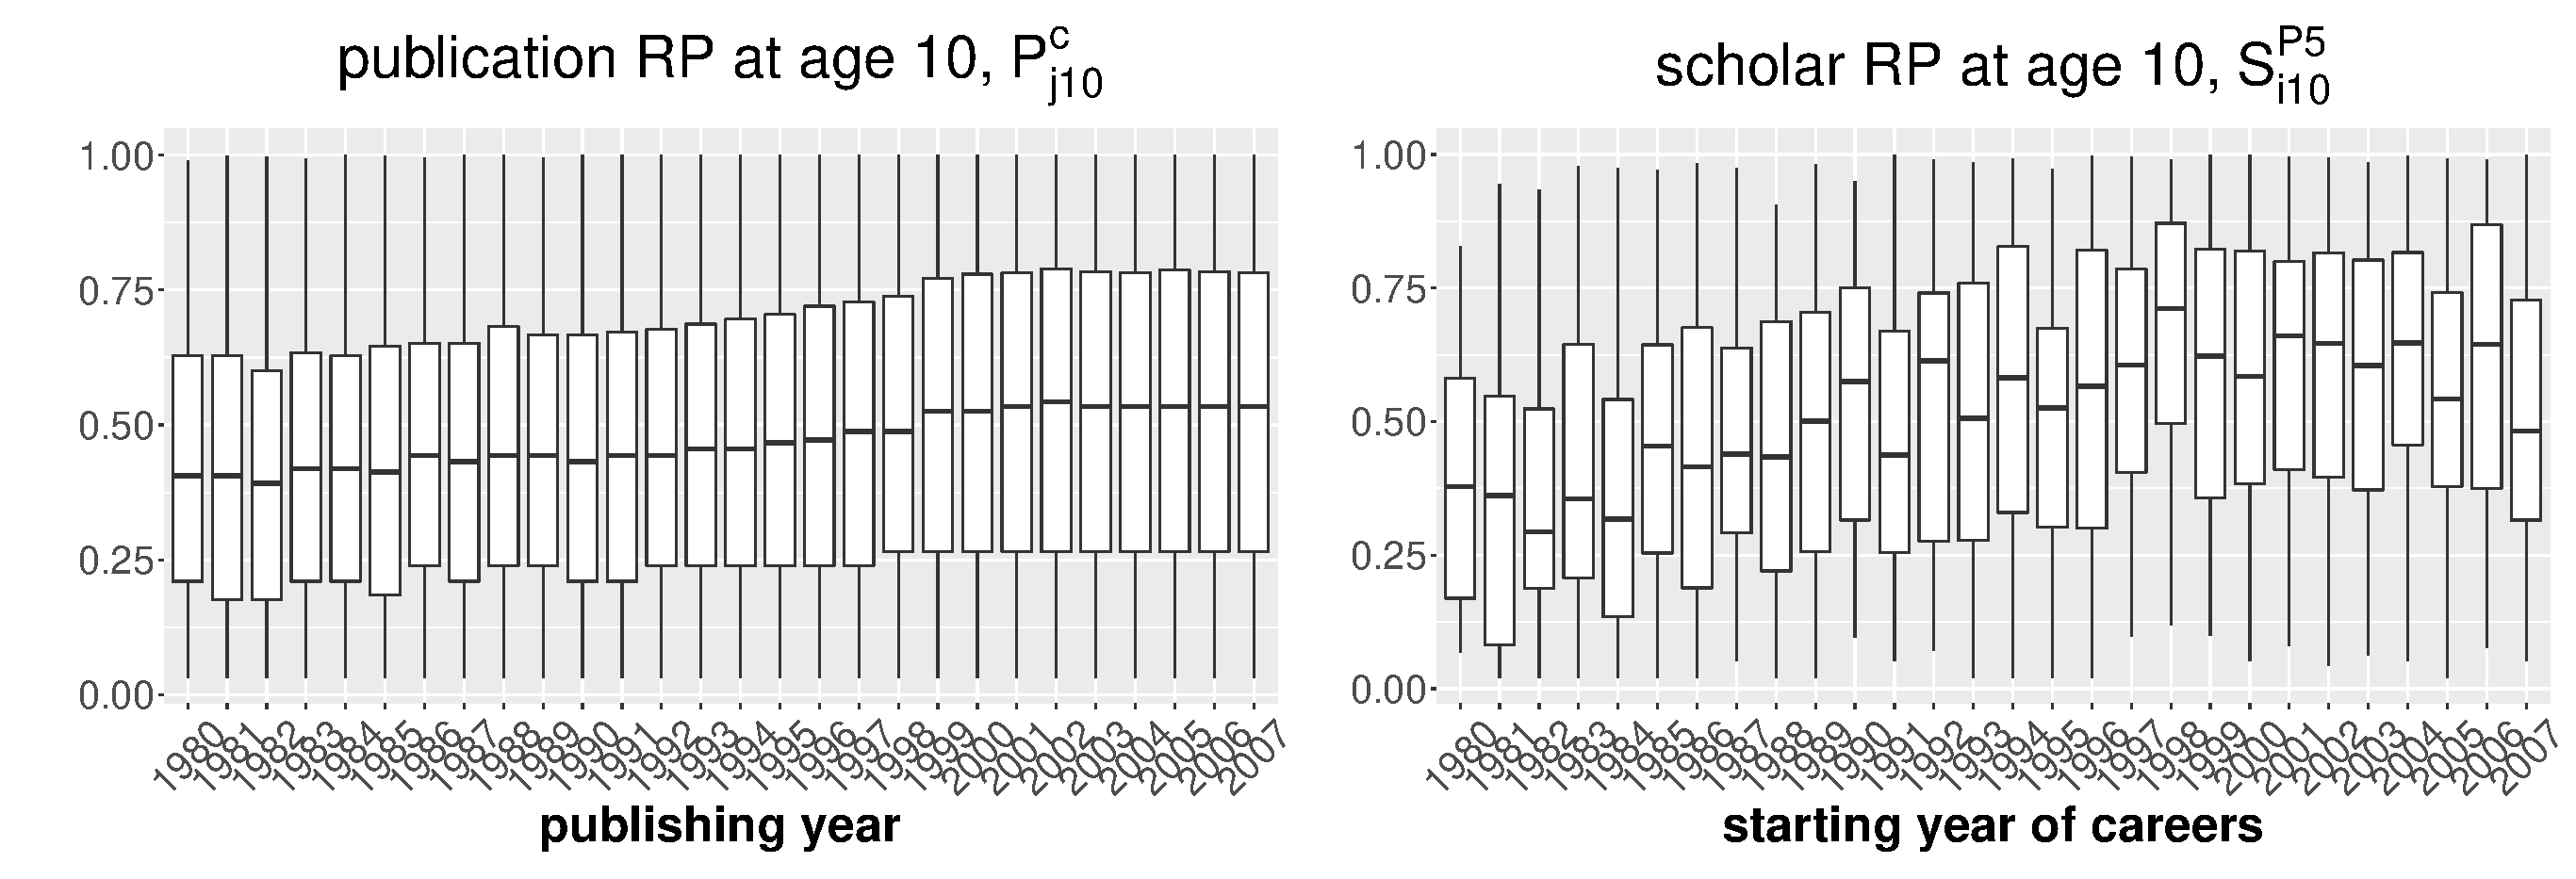
\includegraphics[width=\textwidth]{figures/exploratory/stationarity.eps}
    \caption{P$_{i10}^c$ grouped by the publication years and and S$_{i10}^{P5}$ grouped by the starting years of academic careers. The benchmark contains professors from various disciplines who receive their tenureships in year $2016$ or pubRP .}
    \label{fig:stableness_rp}
\end{figure}


% fig:panos
% show Panos as an example
\begin{figure}[ht!]
    \centering
    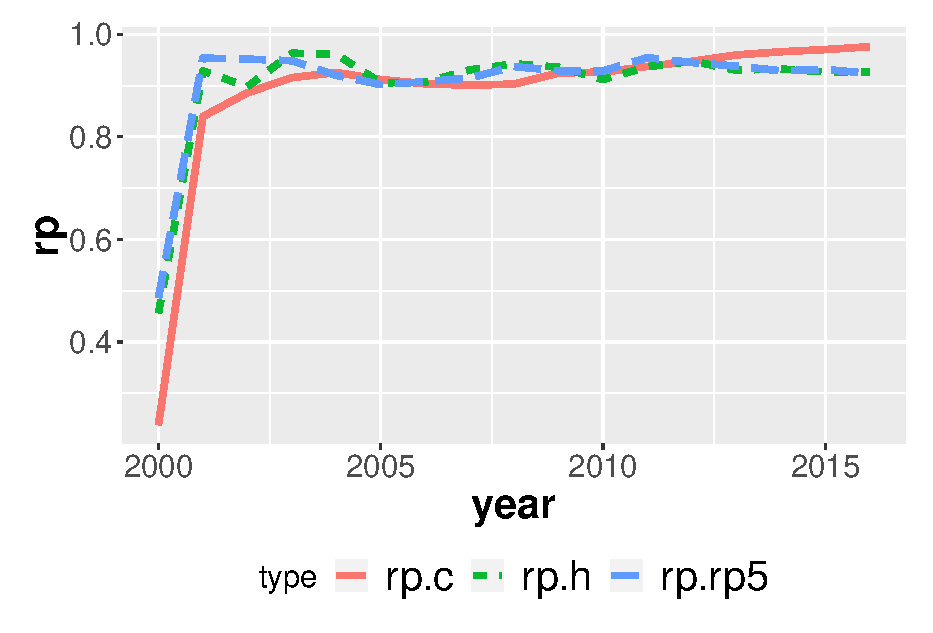
\includegraphics[width=0.7\textwidth]{figures/compare_autrp/panos.eps}
    \caption{The rank percentile indicators for Panos Ipeirotis. The benchmark contains all tenured professors by $2016$.}
    \label{fig:panos}
\end{figure}


% fig:simulated_authors
% show the difference between various author rp
\begin{figure}[ht!]
    \centering
    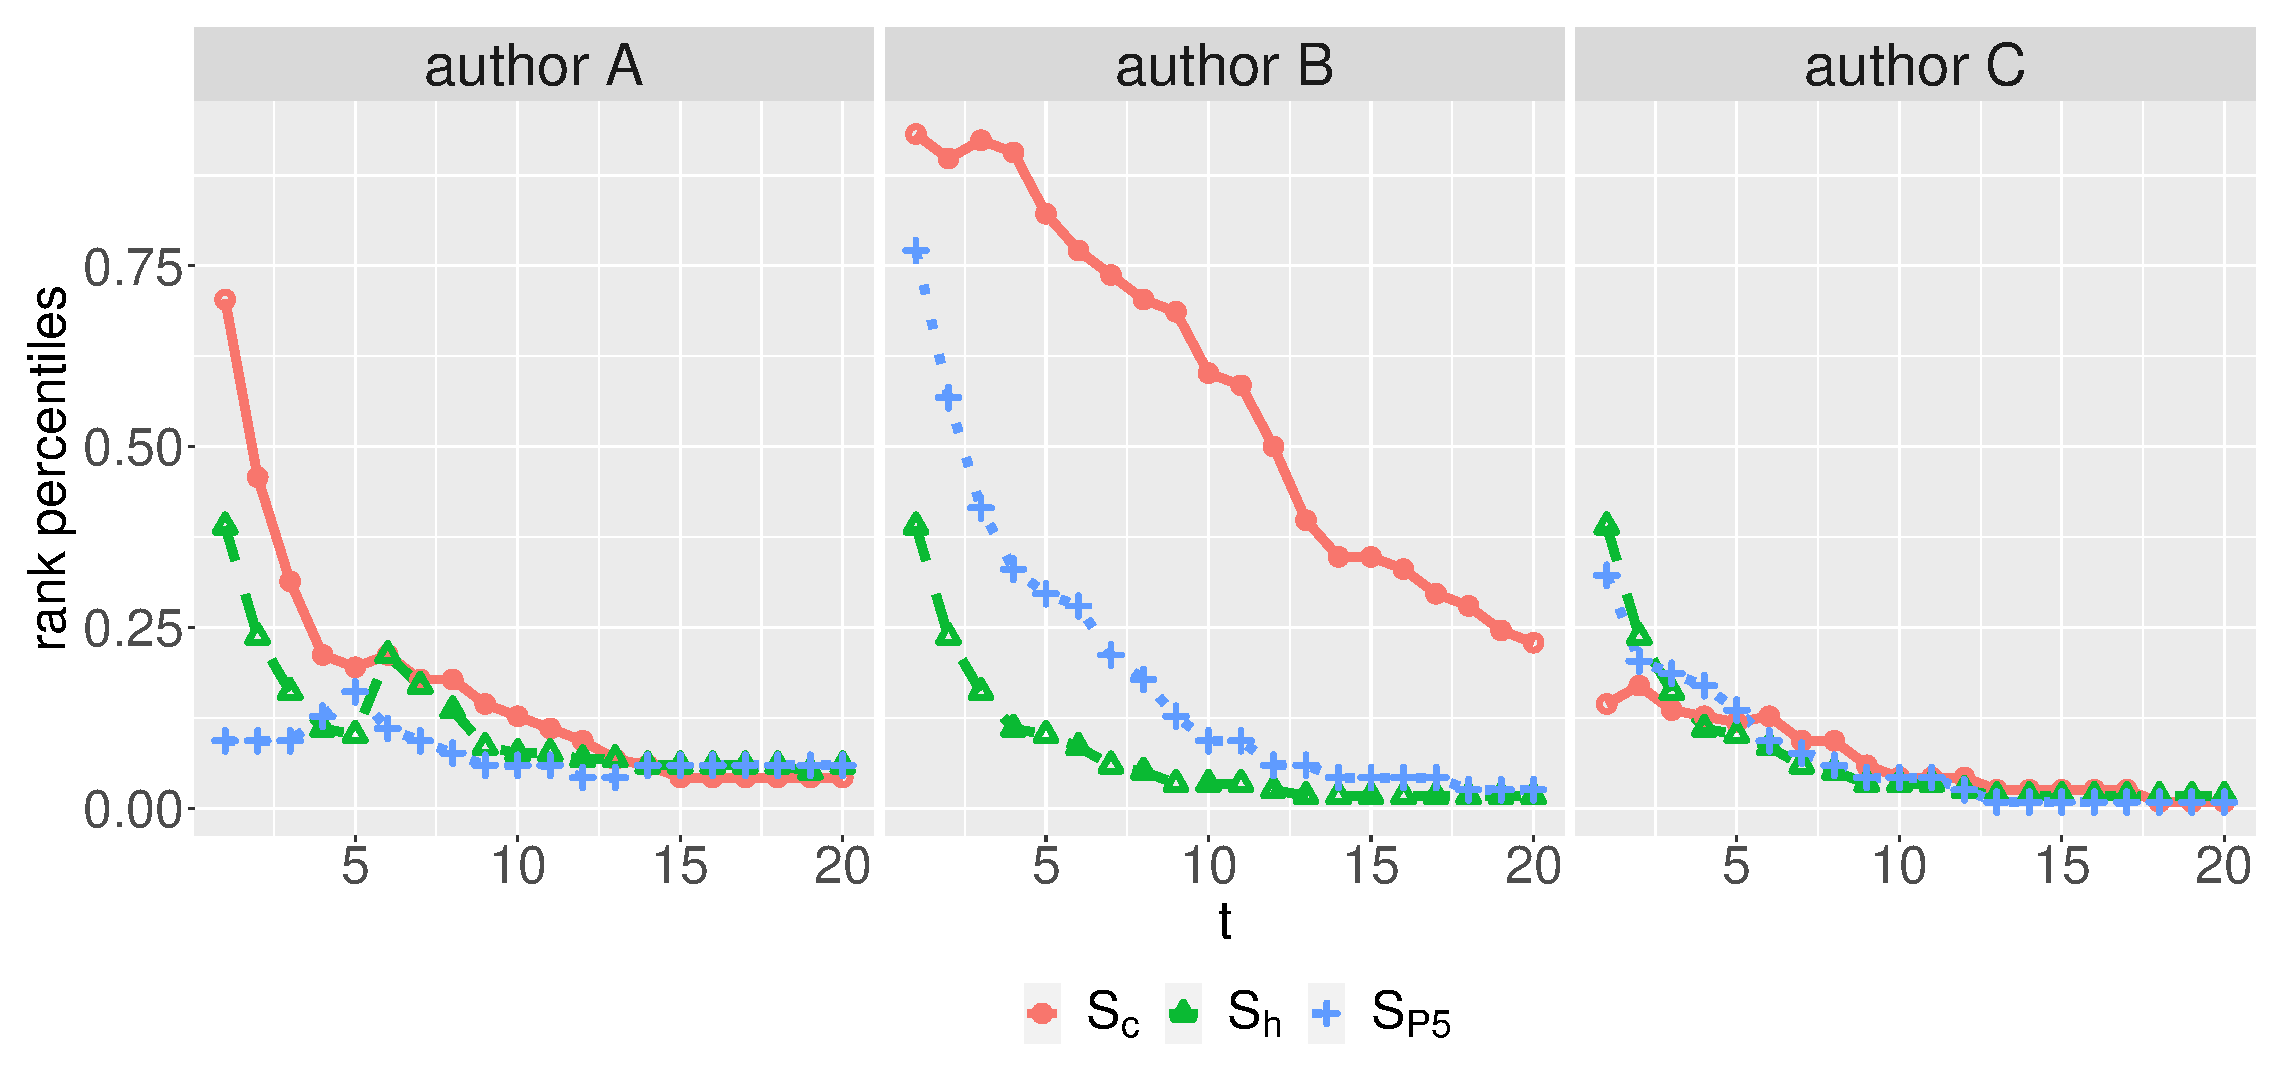
\includegraphics[width=\textwidth]{figures/compare_autrp/simulated_authors.eps}
    \caption{Three artificial authors to illustrate the difference between various types of author rank percentile indicators. Author A is highly productive at all ages but all of the works have little impact. Author B and author C only publish one paper at age $1$ throughout the entire careers, where the paper of author B has very high impact while the paper of author C has medium impact. The h-index of all authors at all ages are $1$. The benchmark contains authors in biology who start their careers from year $1990$.}
    \label{fig:simulated_authors}
\end{figure}


% fig:aut_rp_class
% class agreement among all the author rp
\begin{figure}[ht!]
    \centering
    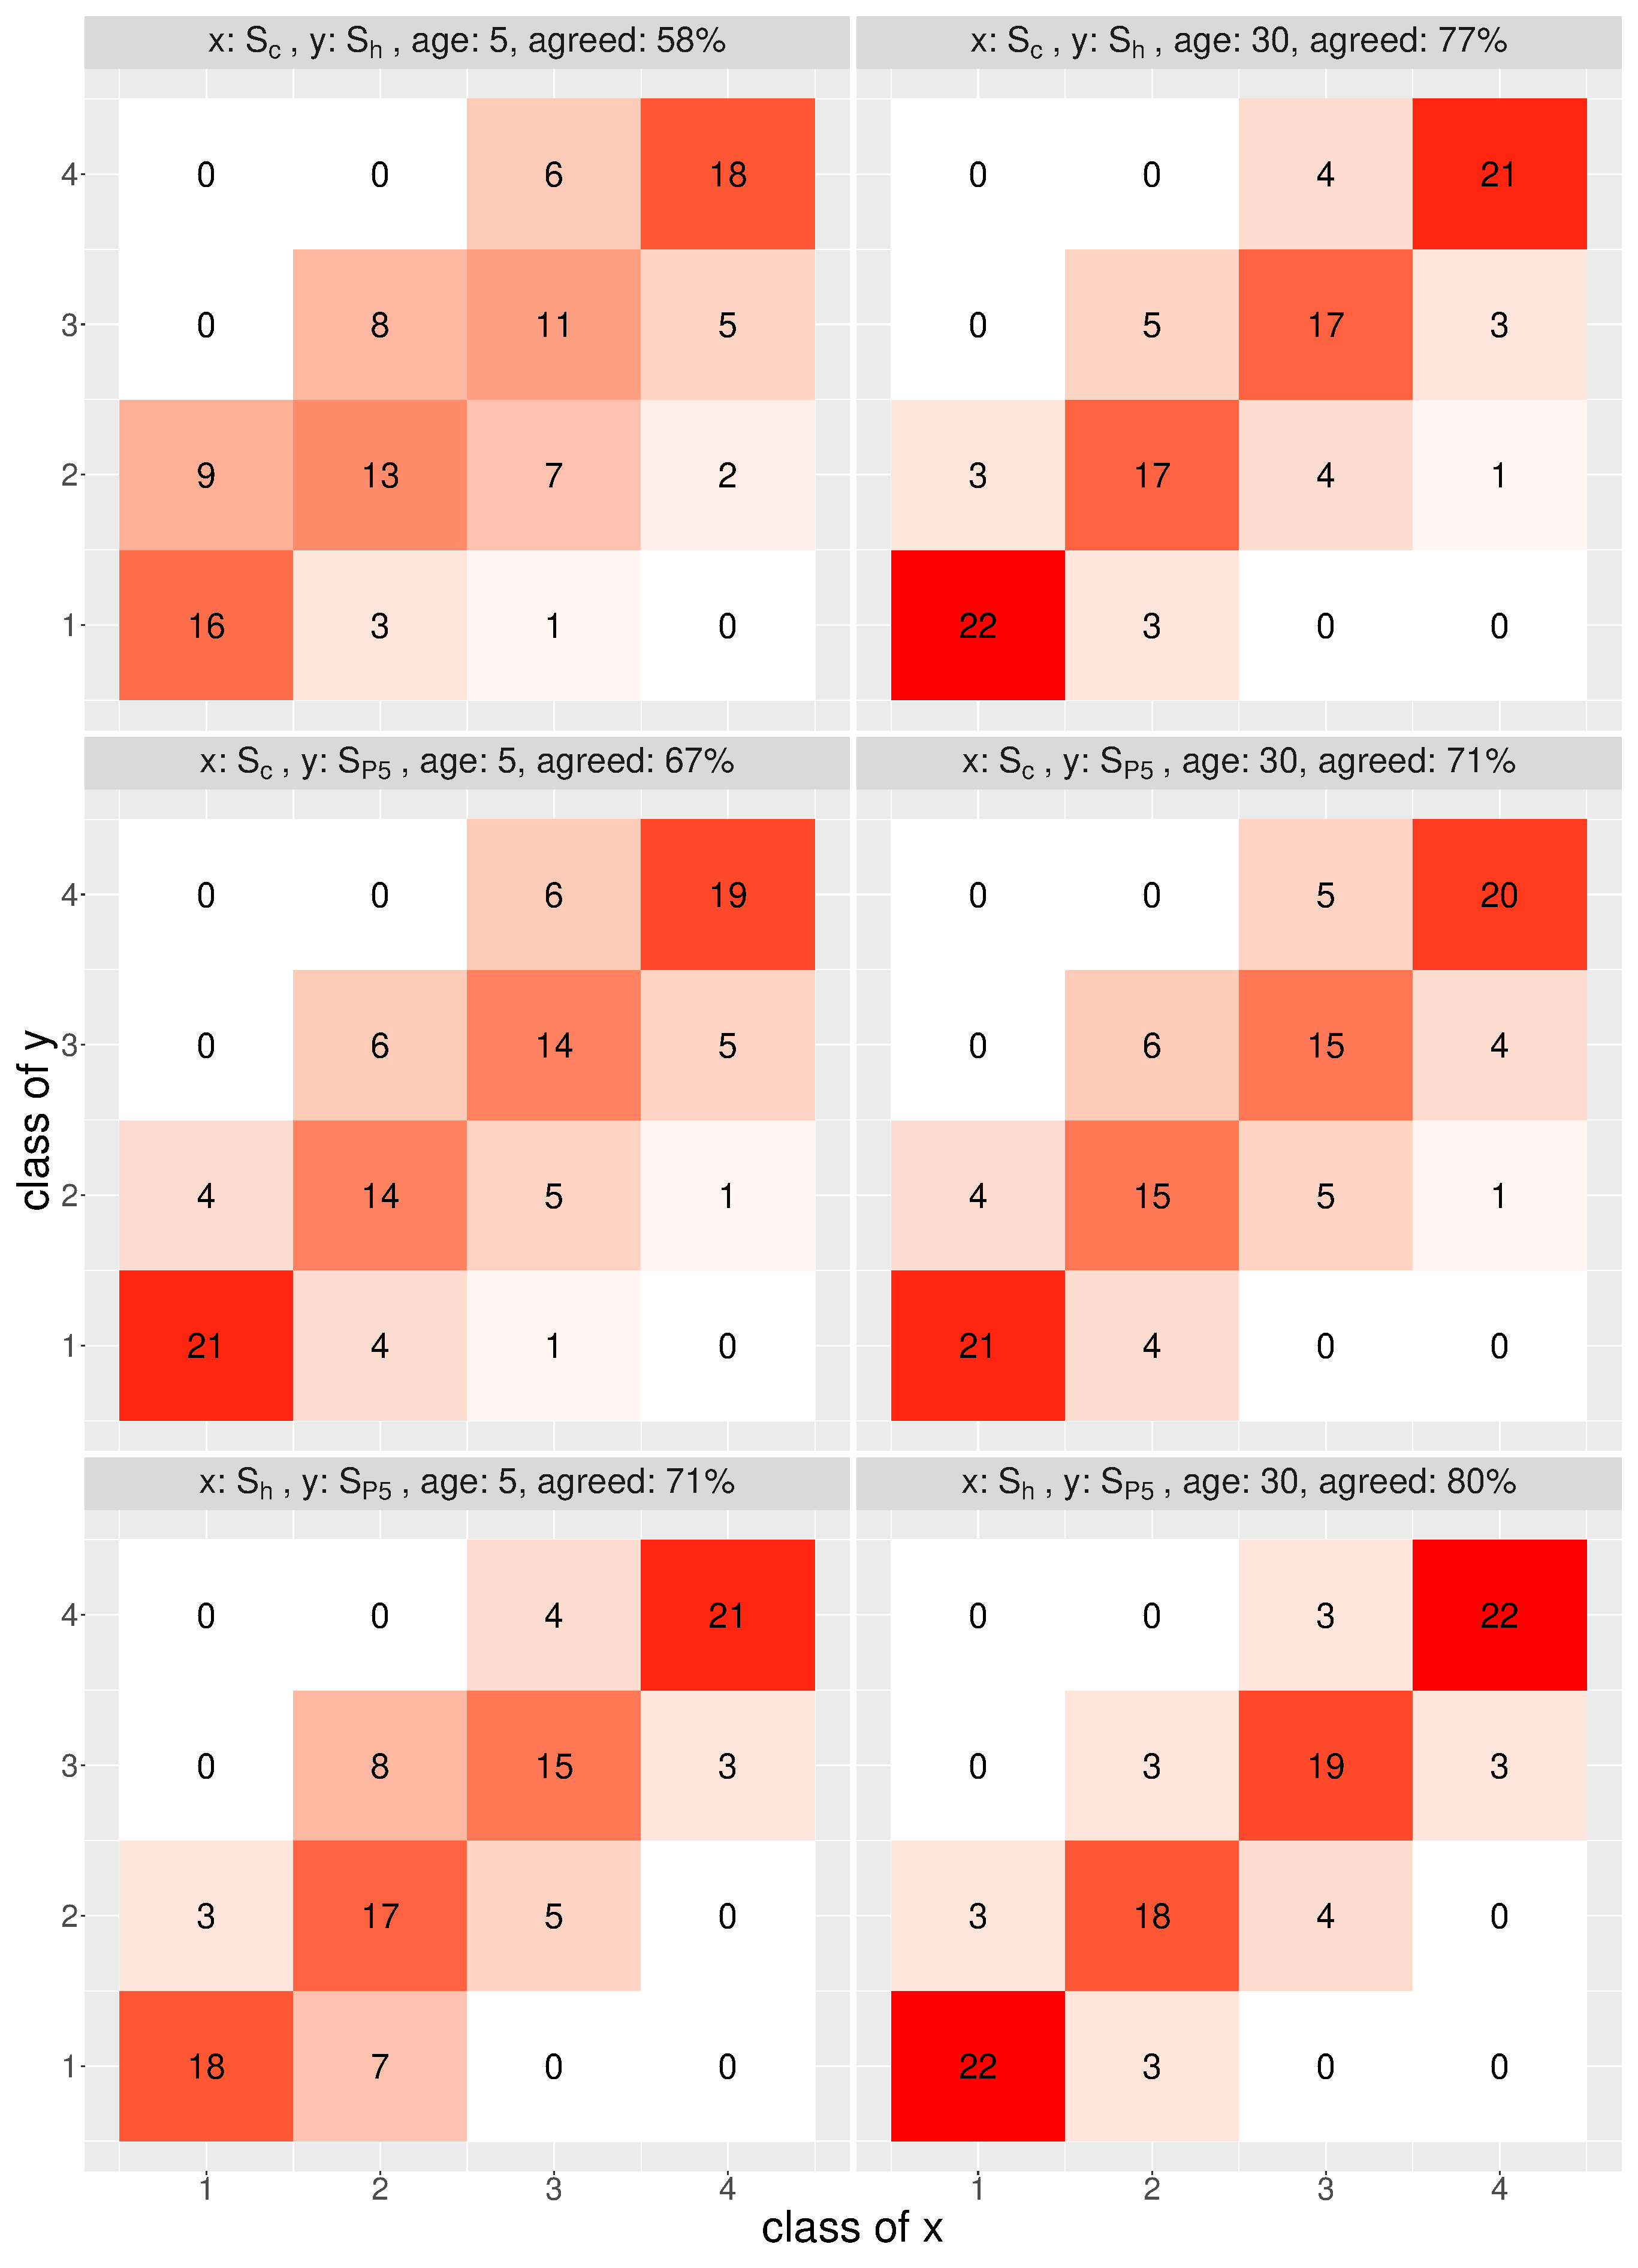
\includegraphics[width=0.88\textwidth]{figures/compare_autrp/heatmap_class_agreement.eps}
    \caption{Classifications of various types of author rp. Each rp is classified into four classes, class 1: $0 \le \text{rp} < 0.25$, class 2: $0.25 \le \text{rp} < 0.5$, class 3: $0.5 \le \text{rp} < 0.75$ and class 4: $0.75 \le \text{rp} \le 1$. The agreement of classifications (sum of the anti-diagonal elements) is displayed in the title of each panel. The benchmark is biology. The agreement for all three types is $51 \%$ at age $5$ and $68 \%$ at age $30$.}
    \label{fig:aut_rp_class}
\end{figure}

% publication rank percentile vs citations, predictability, Wang(2013)
\begin{figure}
     \centering
     \begin{subfigure}[b]{0.48\textwidth}
         \centering
         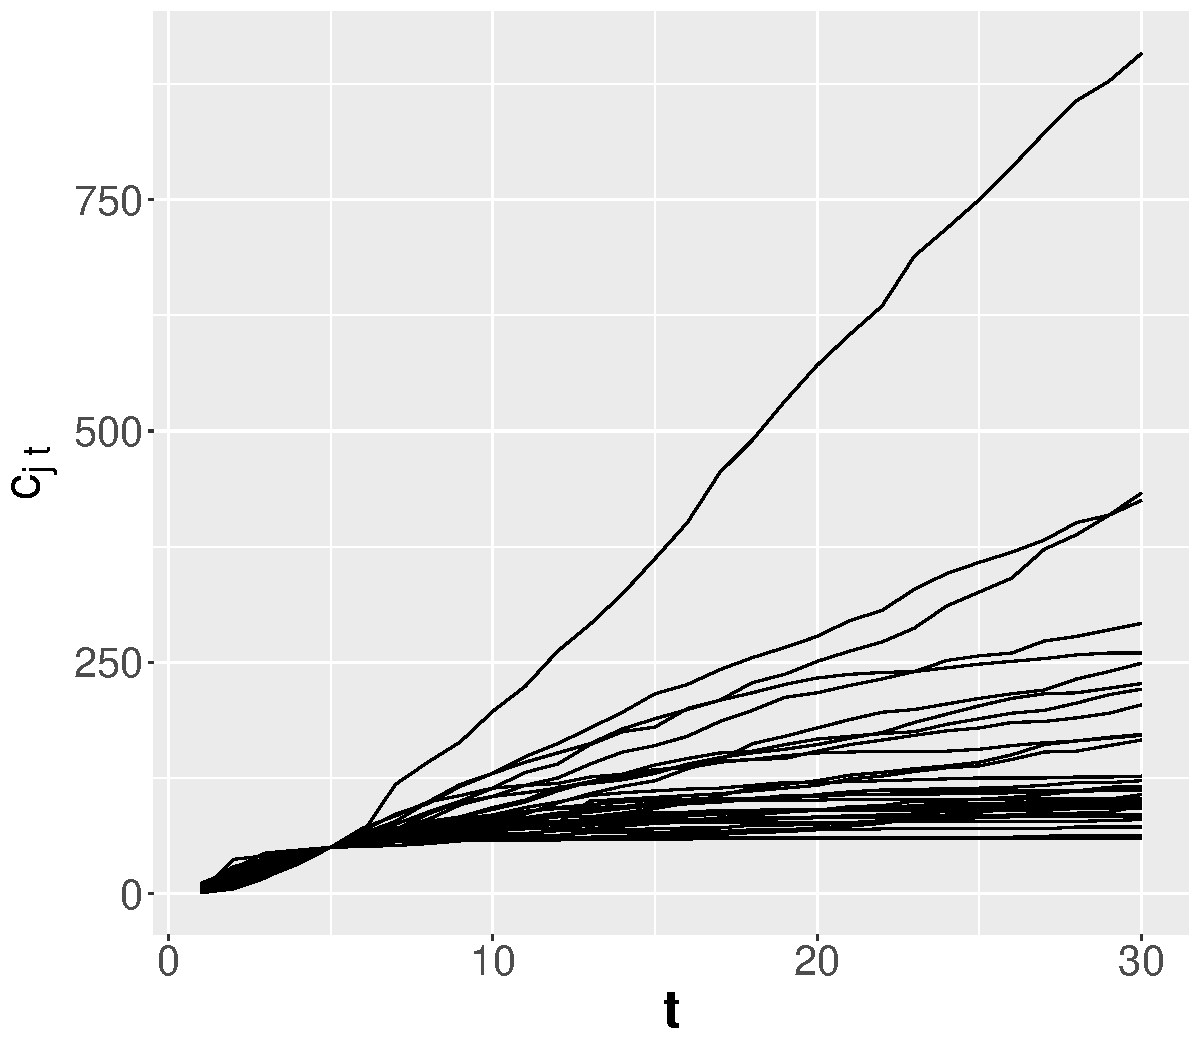
\includegraphics[width=\textwidth]{figures/pred_power/ncit_vs_pubrp/cit_age.pdf}
         \caption{}
         \label{fig:pred_cit_age}
     \end{subfigure}
     \hfill
     \begin{subfigure}[b]{0.48\textwidth}
         \centering
         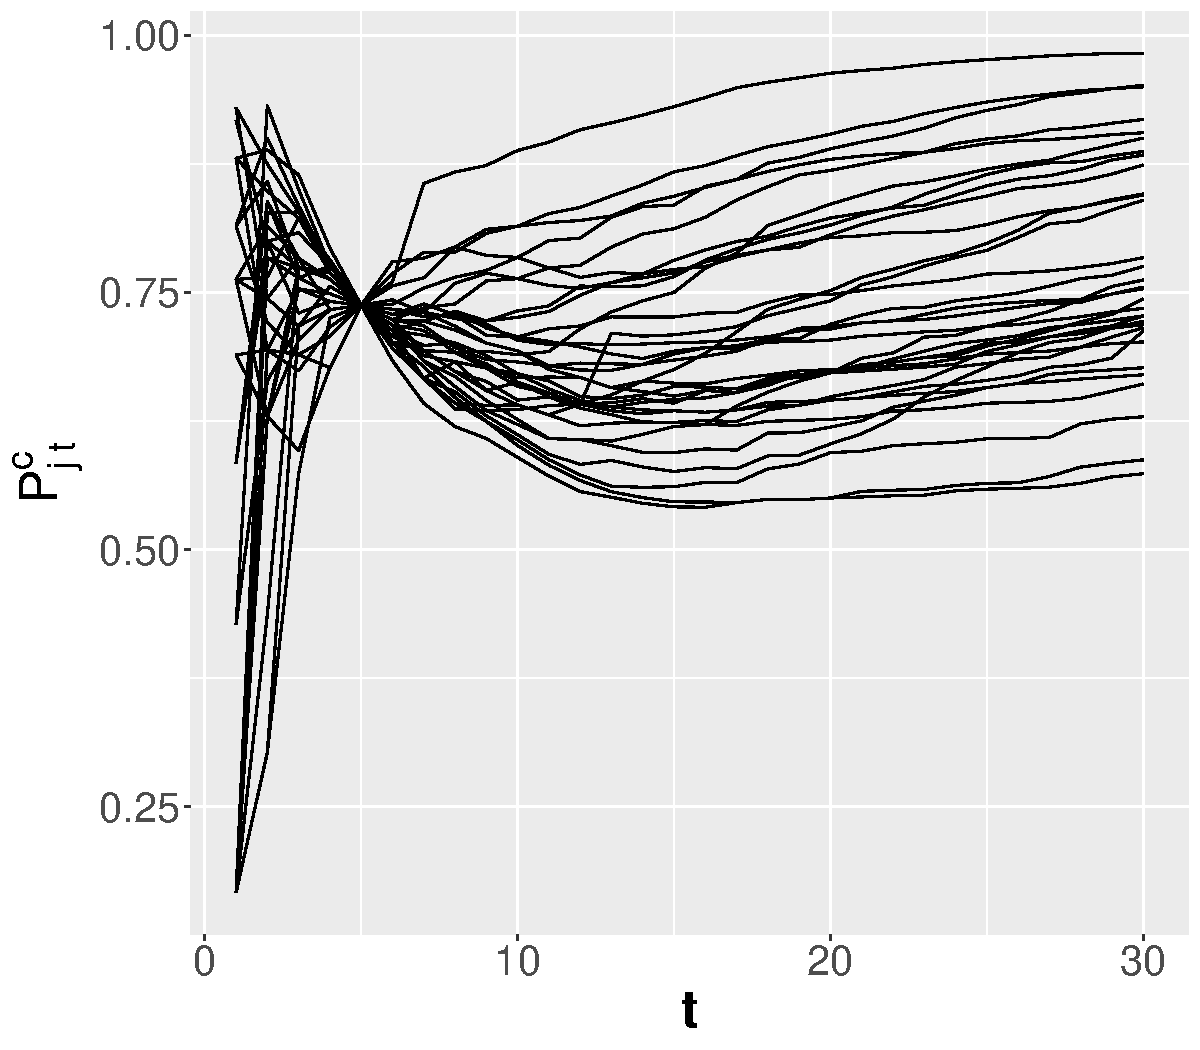
\includegraphics[width=\textwidth]{figures/pred_power/ncit_vs_pubrp/rp_age.pdf}
         \caption{}
         \label{fig:pred_rp_age}
     \end{subfigure}
     \hfill
     \begin{subfigure}[b]{0.48\textwidth}
         \centering
         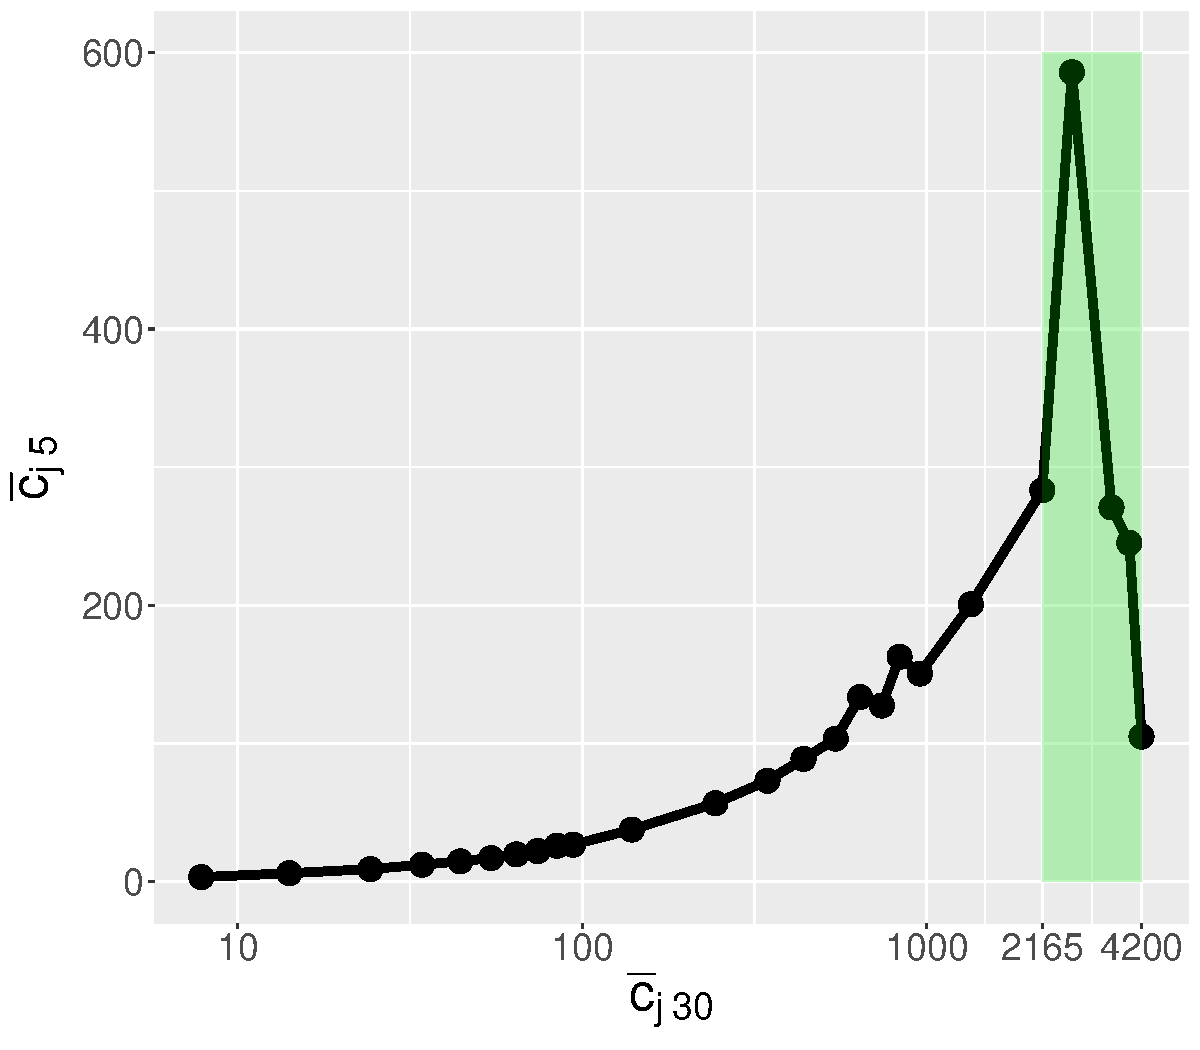
\includegraphics[width=\textwidth]{figures/pred_power/ncit_vs_pubrp/cit_cit.pdf}
         \caption{}
         \label{fig:pred_cit_cit}
     \end{subfigure}
     \hfill
     \begin{subfigure}[b]{0.48\textwidth}
         \centering
         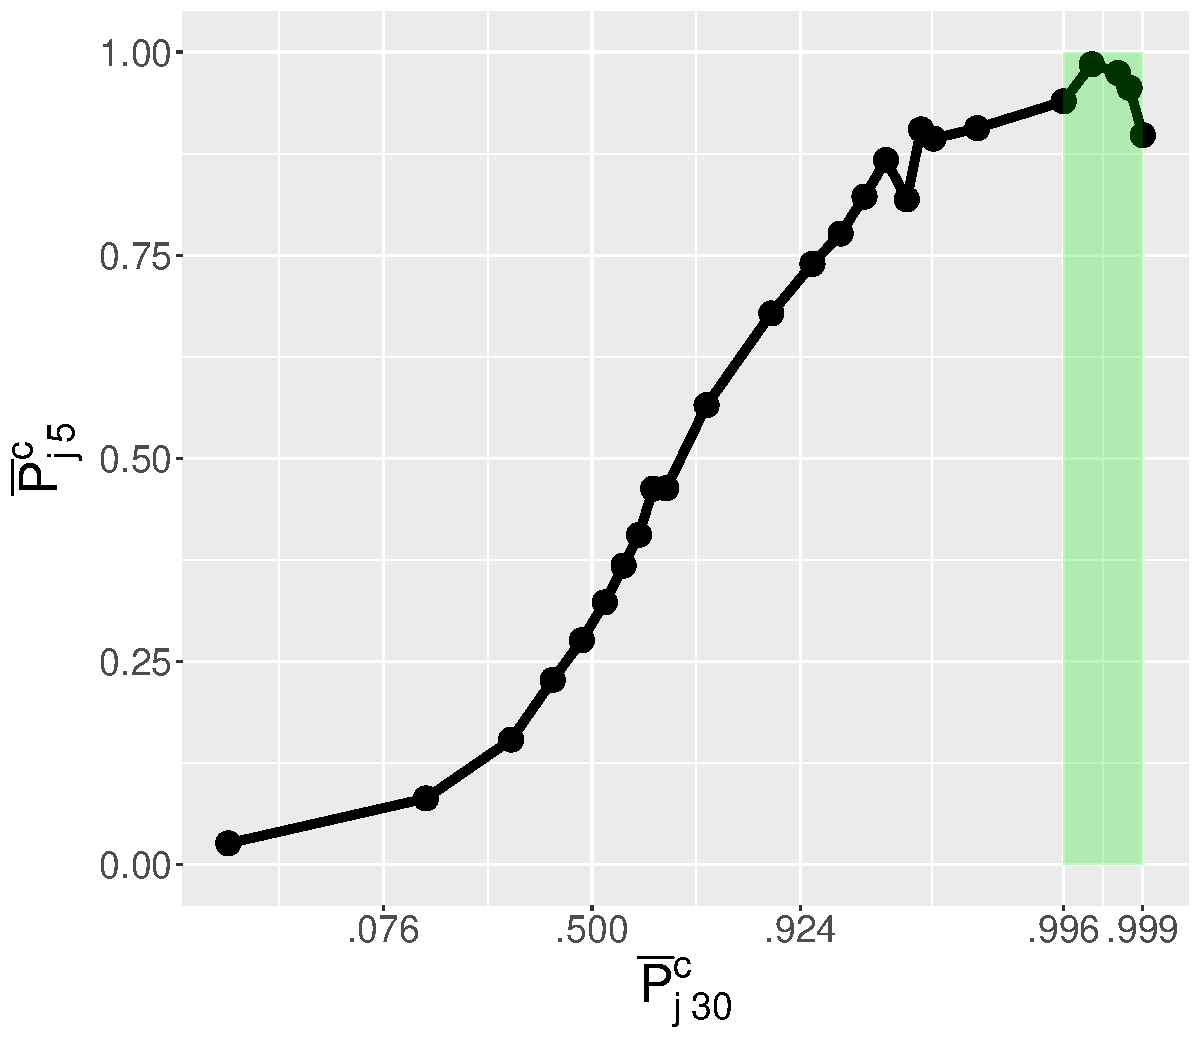
\includegraphics[width=\textwidth]{figures/pred_power/ncit_vs_pubrp/rp_rp.pdf}
         \caption{}
         \label{fig:pred_rp_rp}
     \end{subfigure}
        \caption{The predictability of citations and rank percentiles. The benchmark here is biology. Figure \ref{fig:pred_cit_age} and \ref{fig:pred_rp_age} show the cumulative citations and the corresponding rank percentiles for papers that have $50$ citations by age $5$. Figure \ref{fig:pred_cit_cit} displays the average citations by age $5$ over the average citations by age $30$, for sets of publications, which are pre-specified by dividing the range of $\overline{c_{j 30}}$ into equal intervals in the log scale. Figure \ref{fig:pred_rp_rp} shows the corresponding average rank percentiles for the same sets of publications. Note that we do not claim originality for these plots, as figures \ref{fig:pred_cit_age} and \ref{fig:pred_cit_cit} have been illustrated via a different dataset\supercite{Wang2013}.}
        \label{fig:pub_cit_rp_pred}
\end{figure}


% publication rank percentile, heat map of correlations
\begin{figure}[ht!]
    \centering
    \begin{subfigure}[b]{0.8\textwidth}
        \centering
             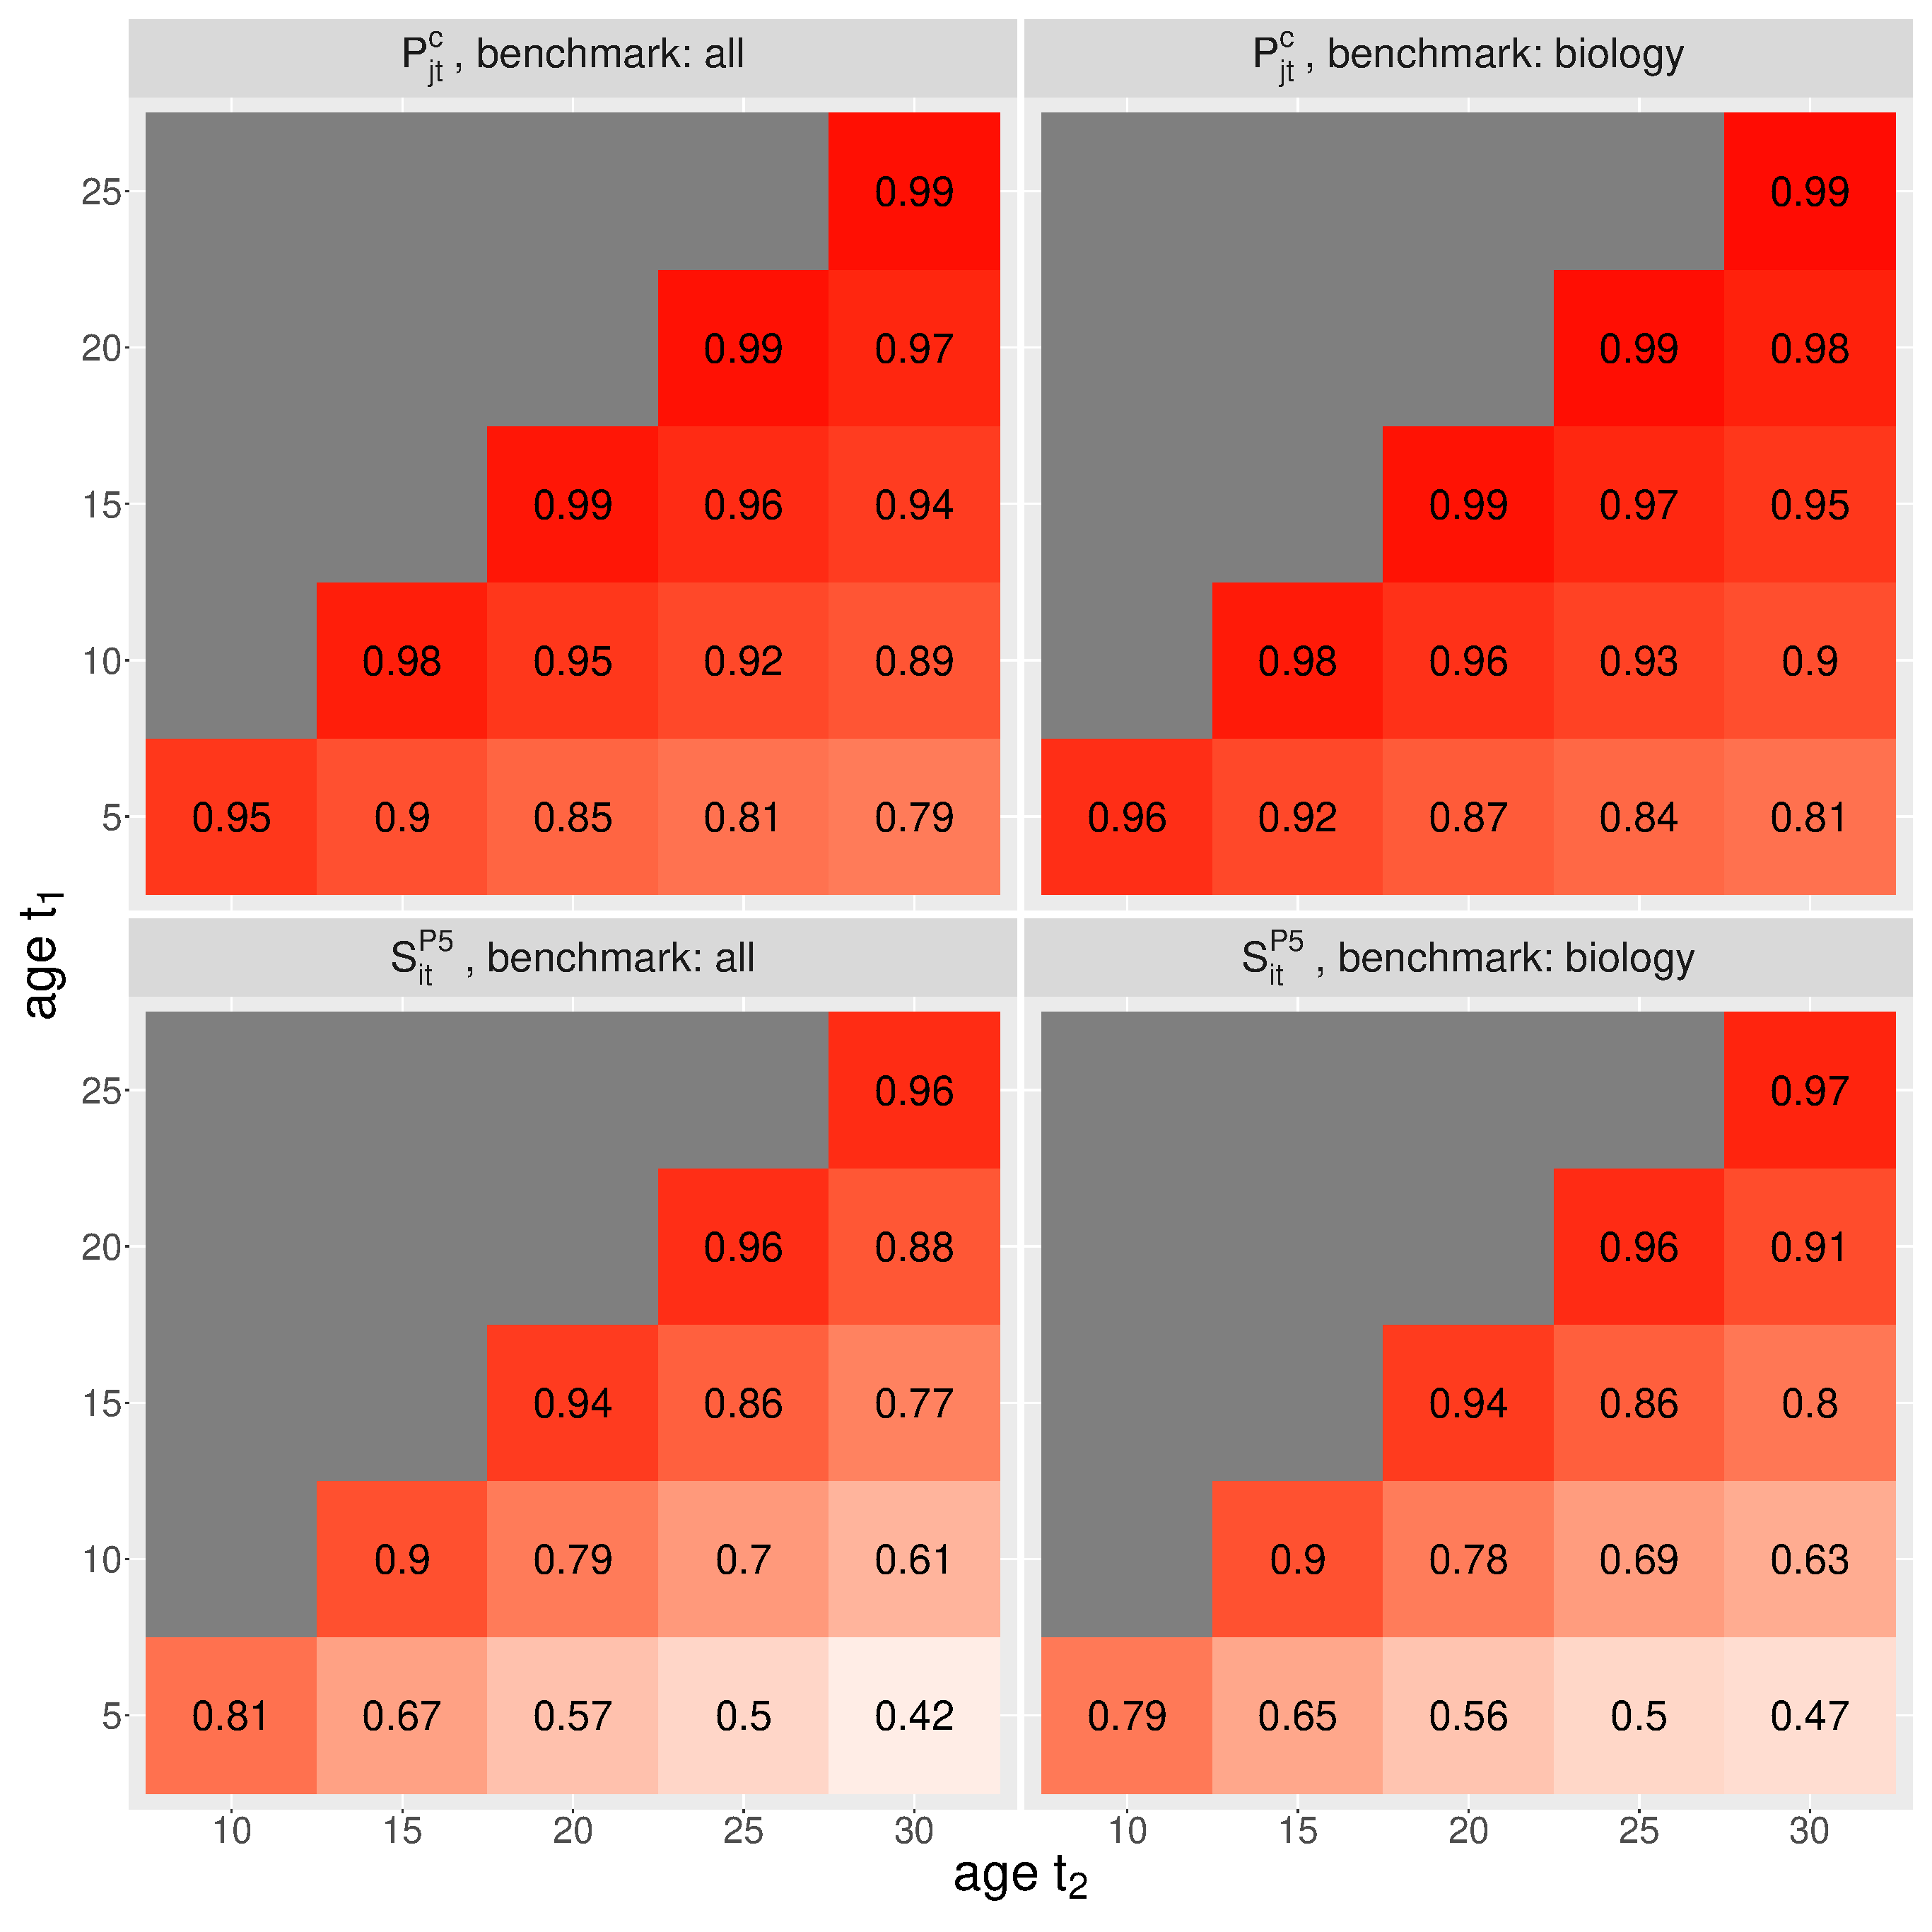
\includegraphics[width=\textwidth]{figures/pred_power/current/heatmap_cor.eps}
         \caption{Predict the cumulative impacts}
         \label{fig:hm_rp_current}
    \end{subfigure}
    
    \begin{subfigure}[b]{0.8\textwidth}
        \centering
             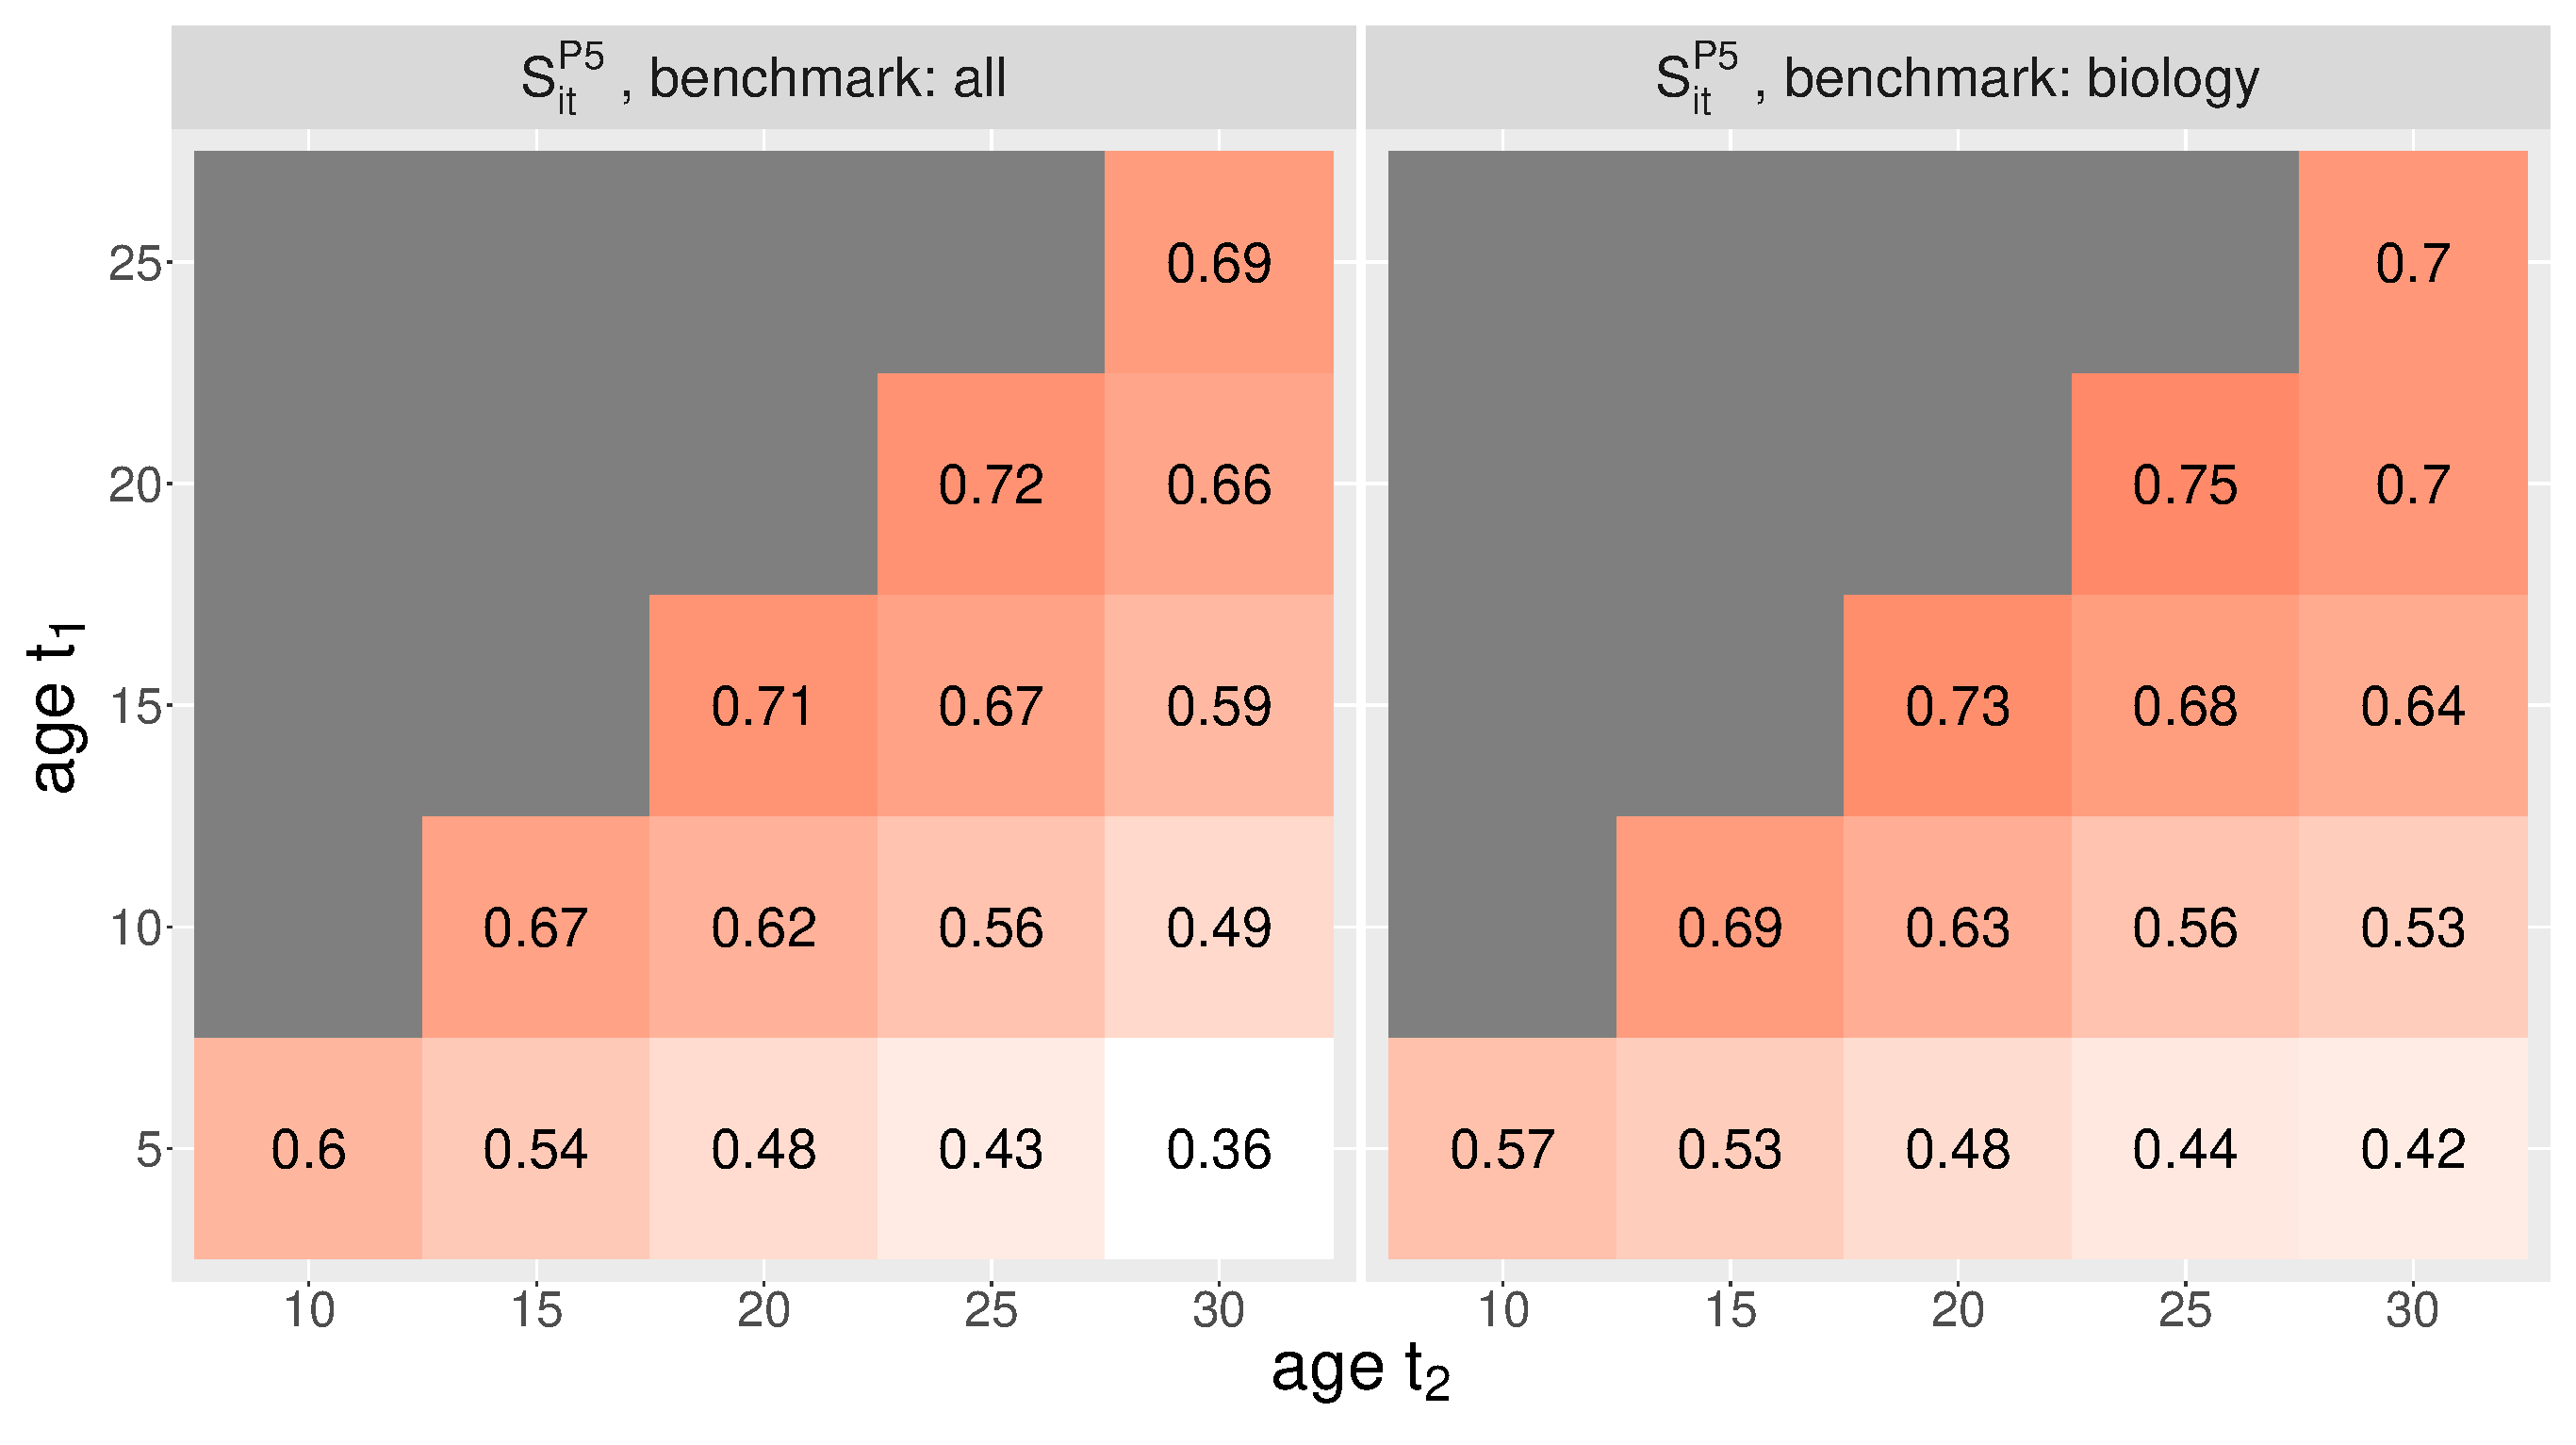
\includegraphics[width=\textwidth]{figures/pred_power/future/heatmap_cor.eps}
         \caption{Predict the future scientific output}
         \label{fig:hm_rp_future}
    \end{subfigure}
    \caption{The Pearson's correlation between rp indicators at two different ages. }
    \label{fig:hm_rp}
\end{figure}
\begin{figure}[ht!]
    \centering
    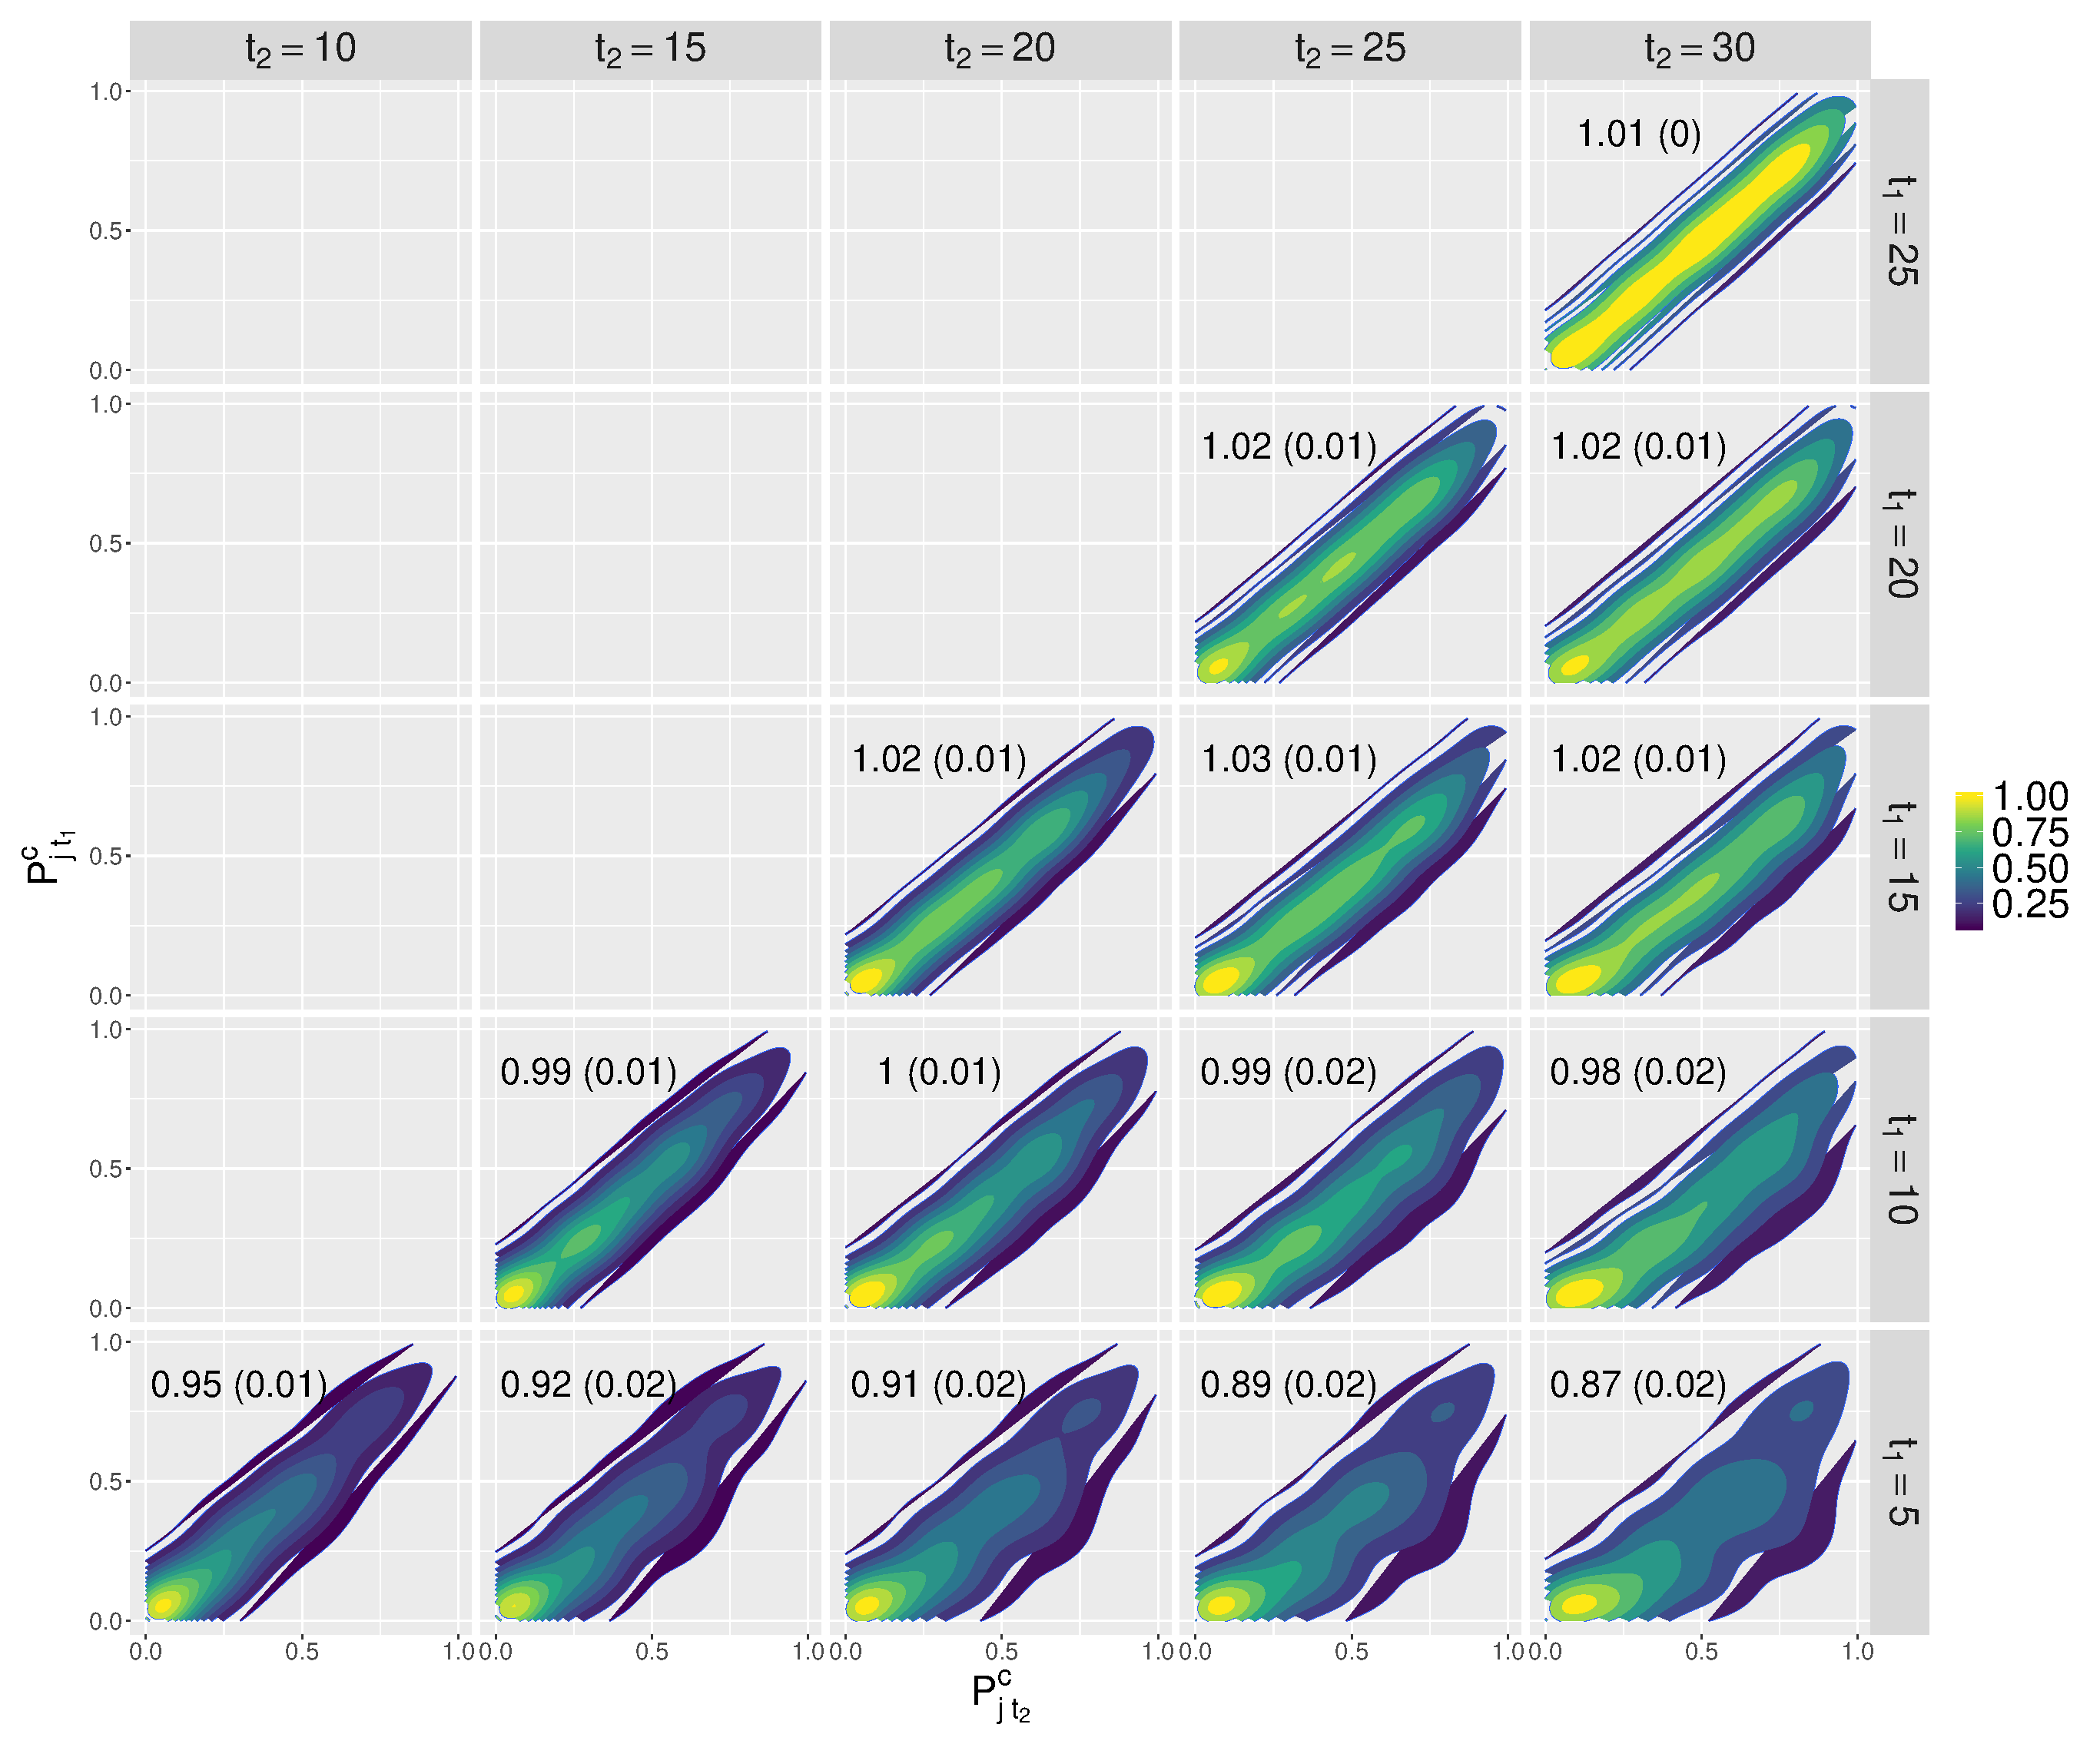
\includegraphics[width=\textwidth]{figures/pred_power/pubrp/scatter_bio1980.eps}
    \caption{Kernel density estimation of the scatters of rp.c$_{\cdot \tau_1}$ and rp.c$_{\cdot \tau_2}$. Meanwhile, we fit a simple linear regression of rp.c$_{\cdot \tau_2}$ upon rp.c$_{\cdot \tau_1}$. The estimated coefficient of rp.c$_{\cdot \tau_1}$ and the corresponding standard error (in the bracket) are displayed in each facet. The benchmark here includes all publications in biology and written in $1980$.}
    \label{fig:scatter_pubrp_bio1980}
\end{figure}

\iffalse
% author rank percentile, heat map of correlations
\begin{figure}[ht!]
    \centering
    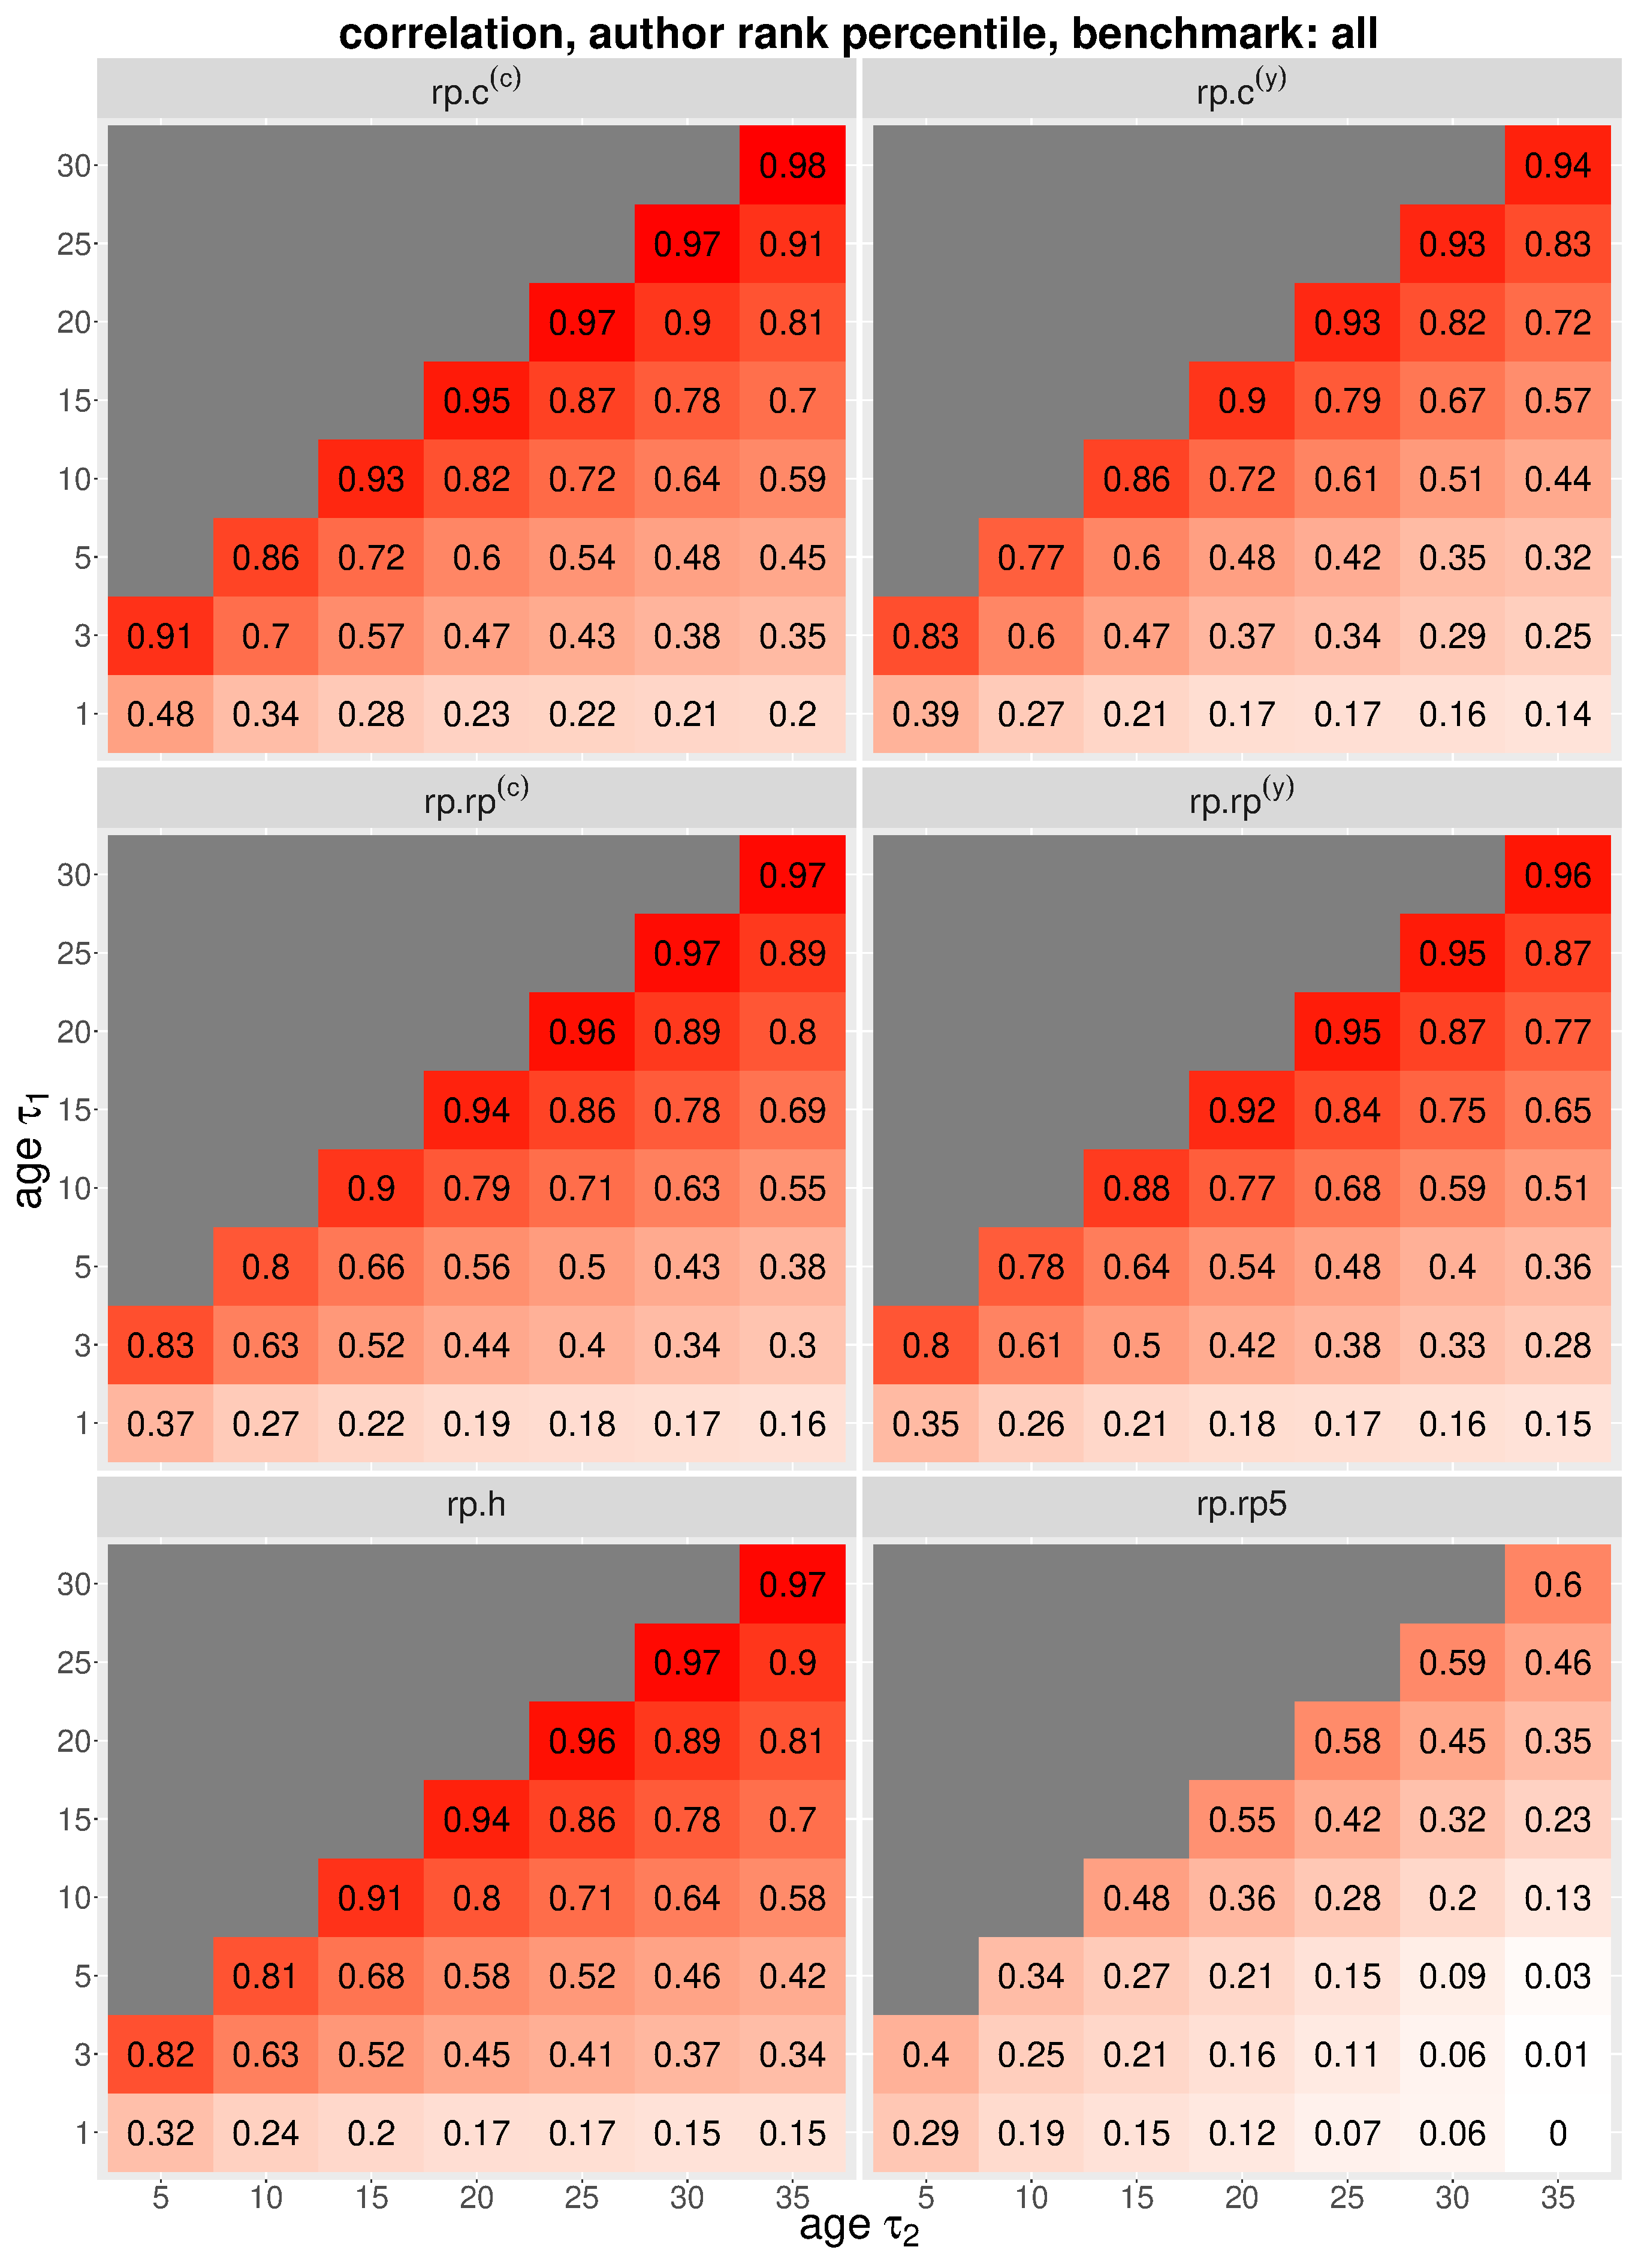
\includegraphics[width=\textwidth]{figures/pred_power/autrp/heatmap_cor_all.eps}
    \caption{The Pearson's correlation between rp at two different ages, for various types of author rp. The benchmark includes all the authors.}
    \label{fig:hm_autrp_all}
\end{figure}
\begin{figure}[ht!]
    \centering
    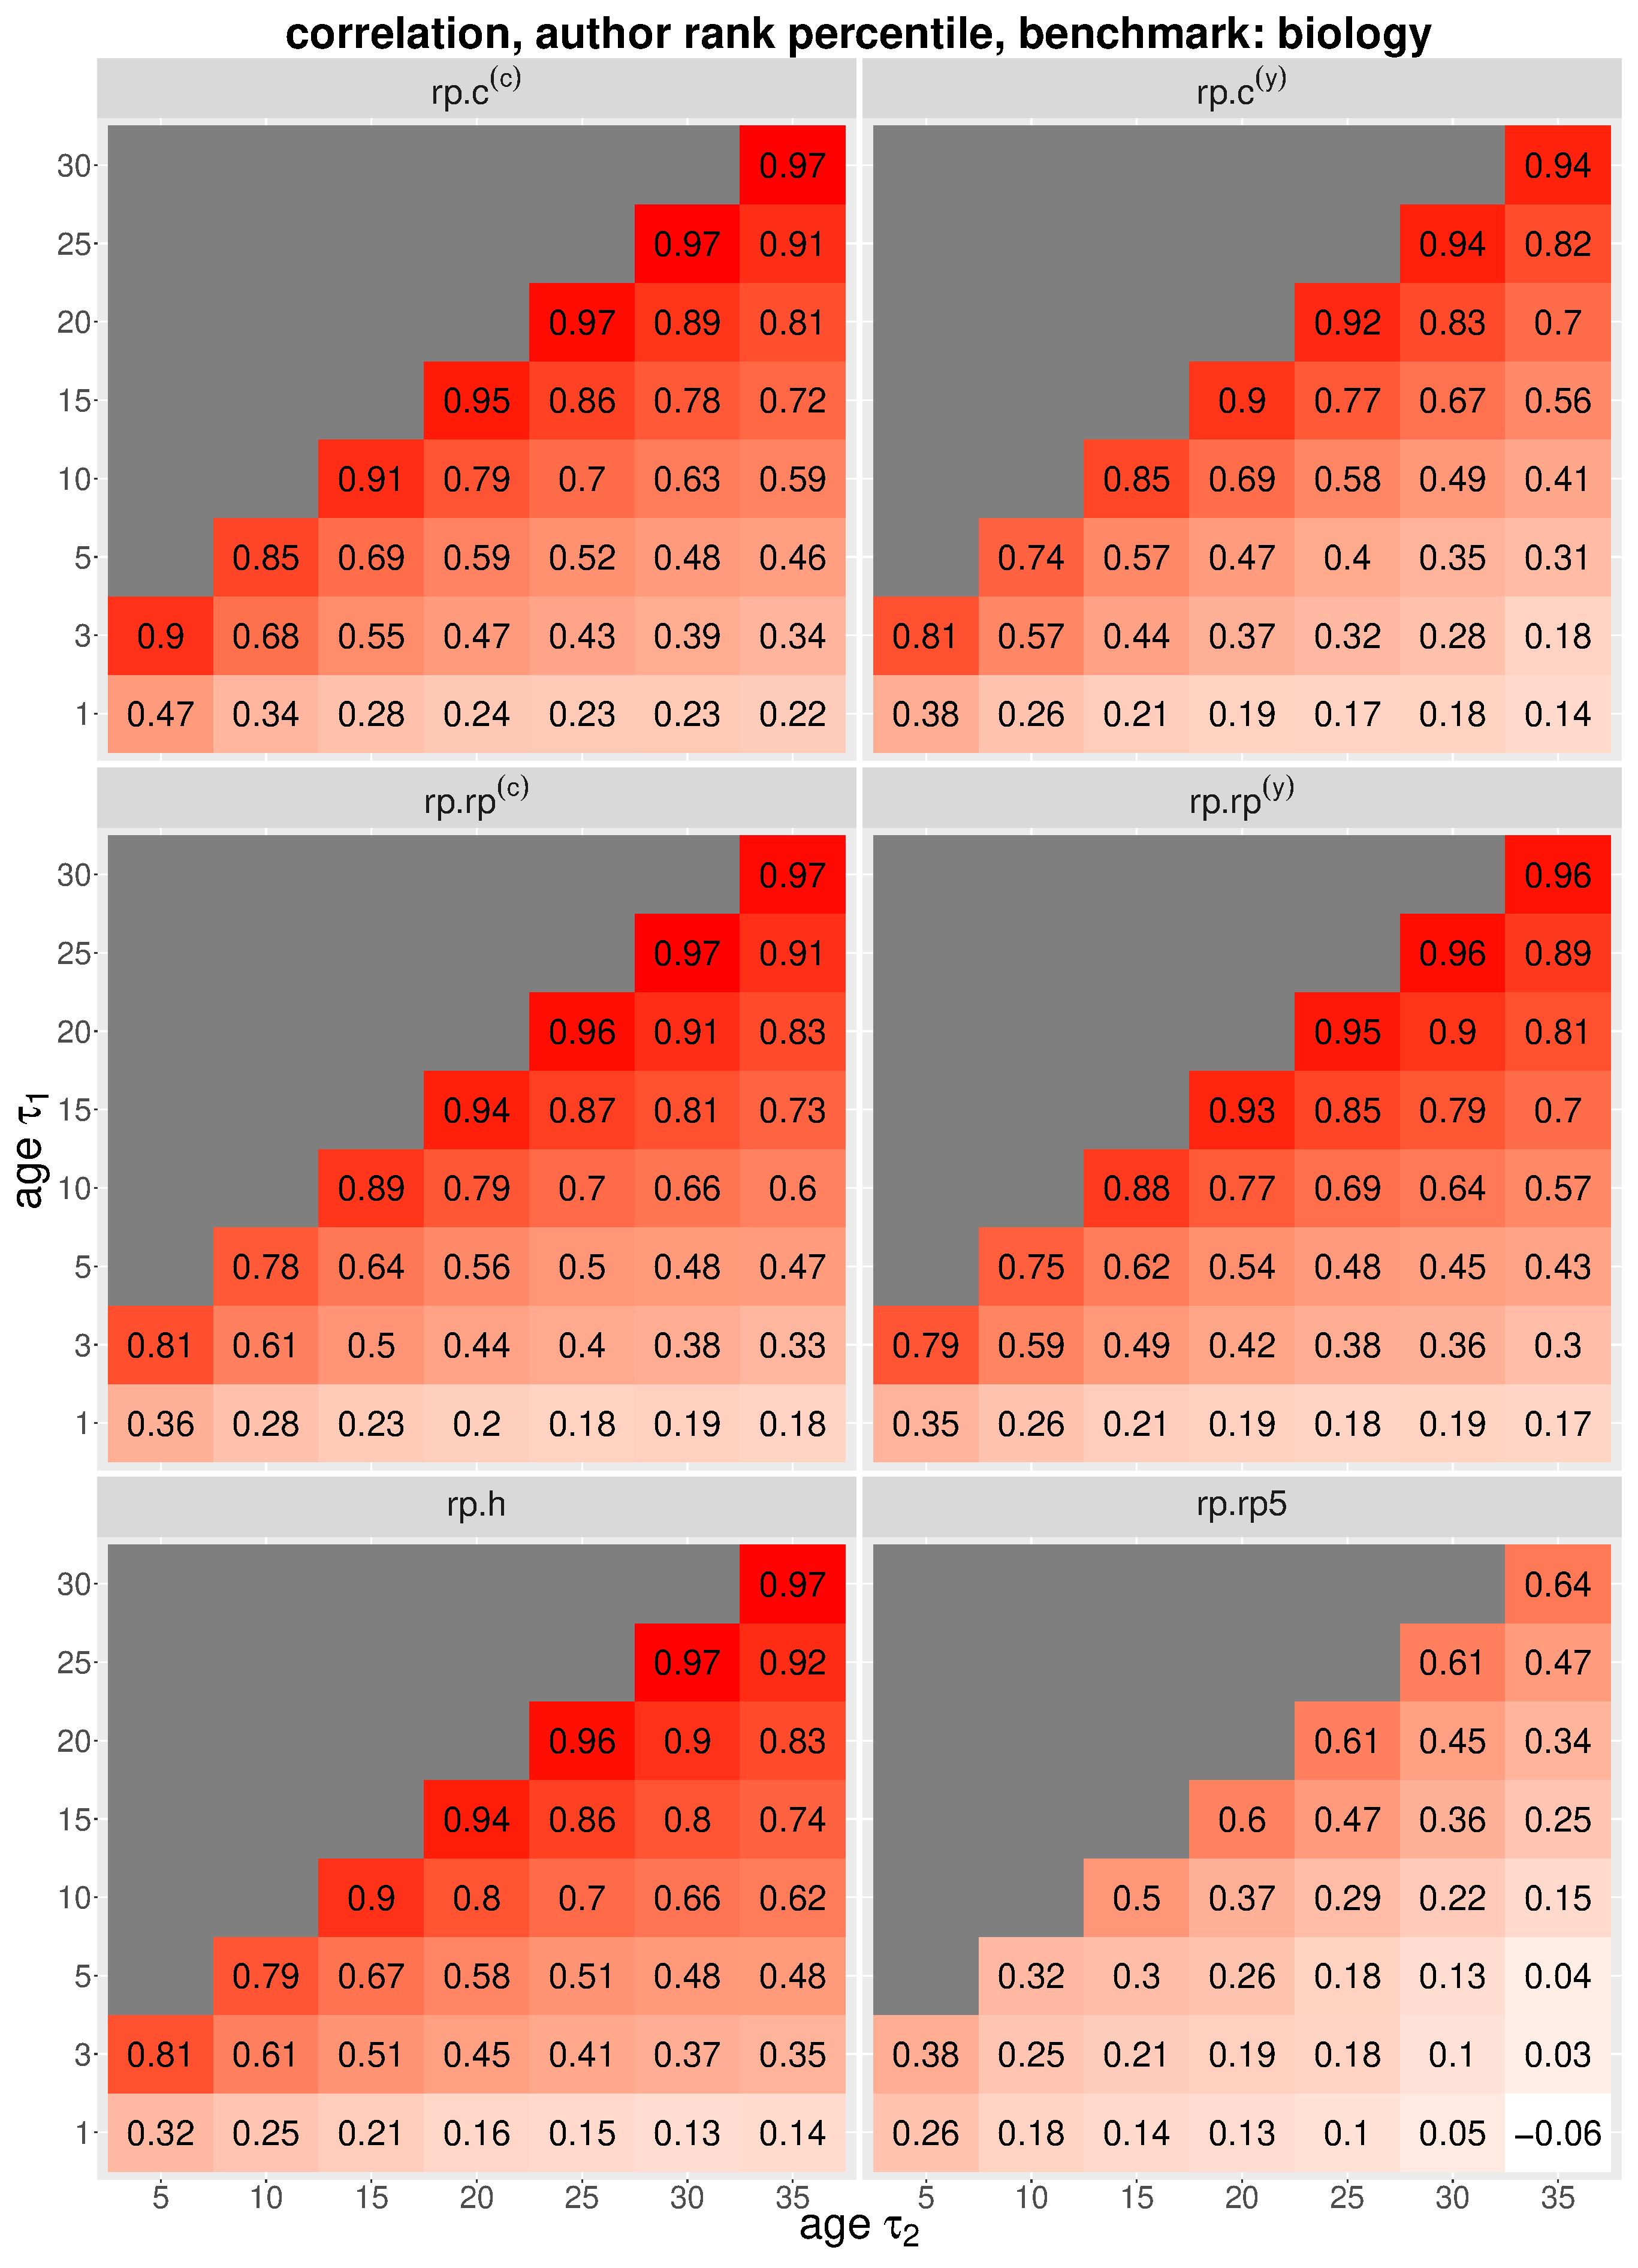
\includegraphics[width=\textwidth]{figures/pred_power/autrp/heatmap_cor_bio.eps}
    \caption{The Pearson's correlation between rp at two different ages, for various types of author rp. The benchmark includes only authors in biology.}
    \label{fig:hm_autrp_biology}
\end{figure}

\begin{figure}[ht!]
    \centering
    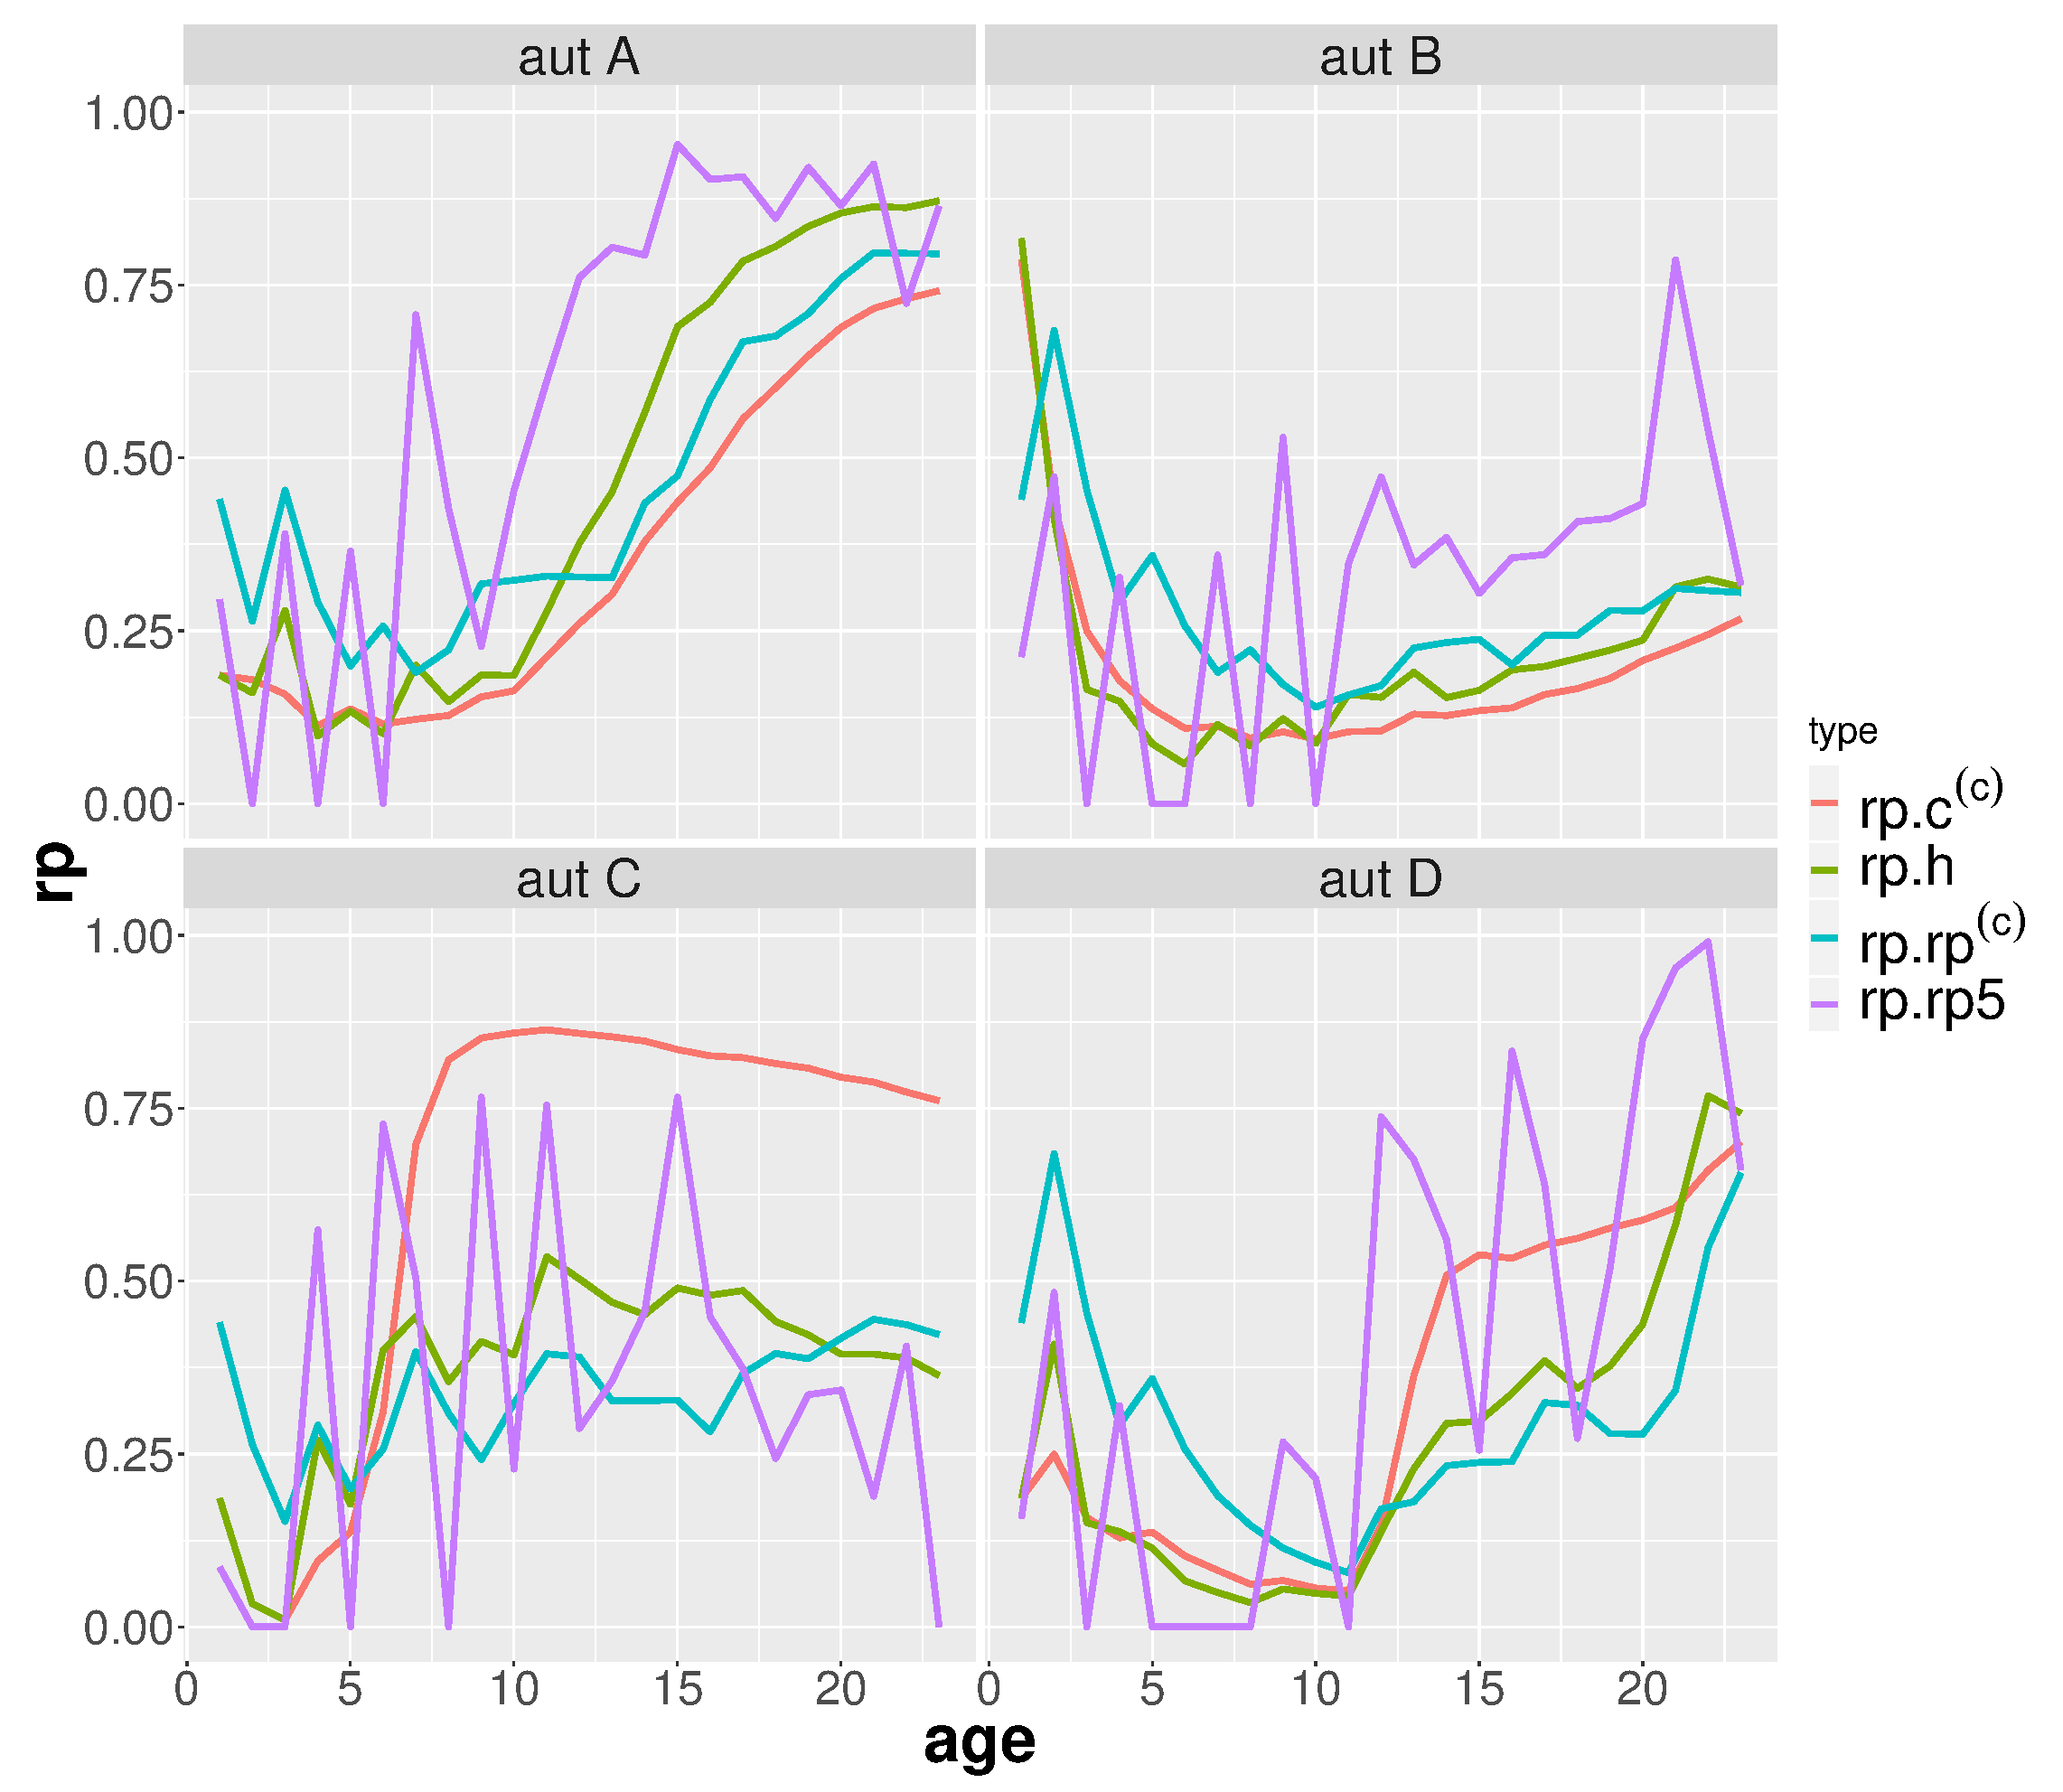
\includegraphics[width=\textwidth]{figures/exploratory/autrp_examples.eps}
    \caption{Examples of various types of author rank percentile over age. The $4$ authors shown in the figure have the same $\text{rp}^{(c)}_{i 5}$ and are all starting their careers from year $1990$. }
    \label{fig:aut_examples}
\end{figure}
\fi

\begin{figure}[ht!]
    \centering
    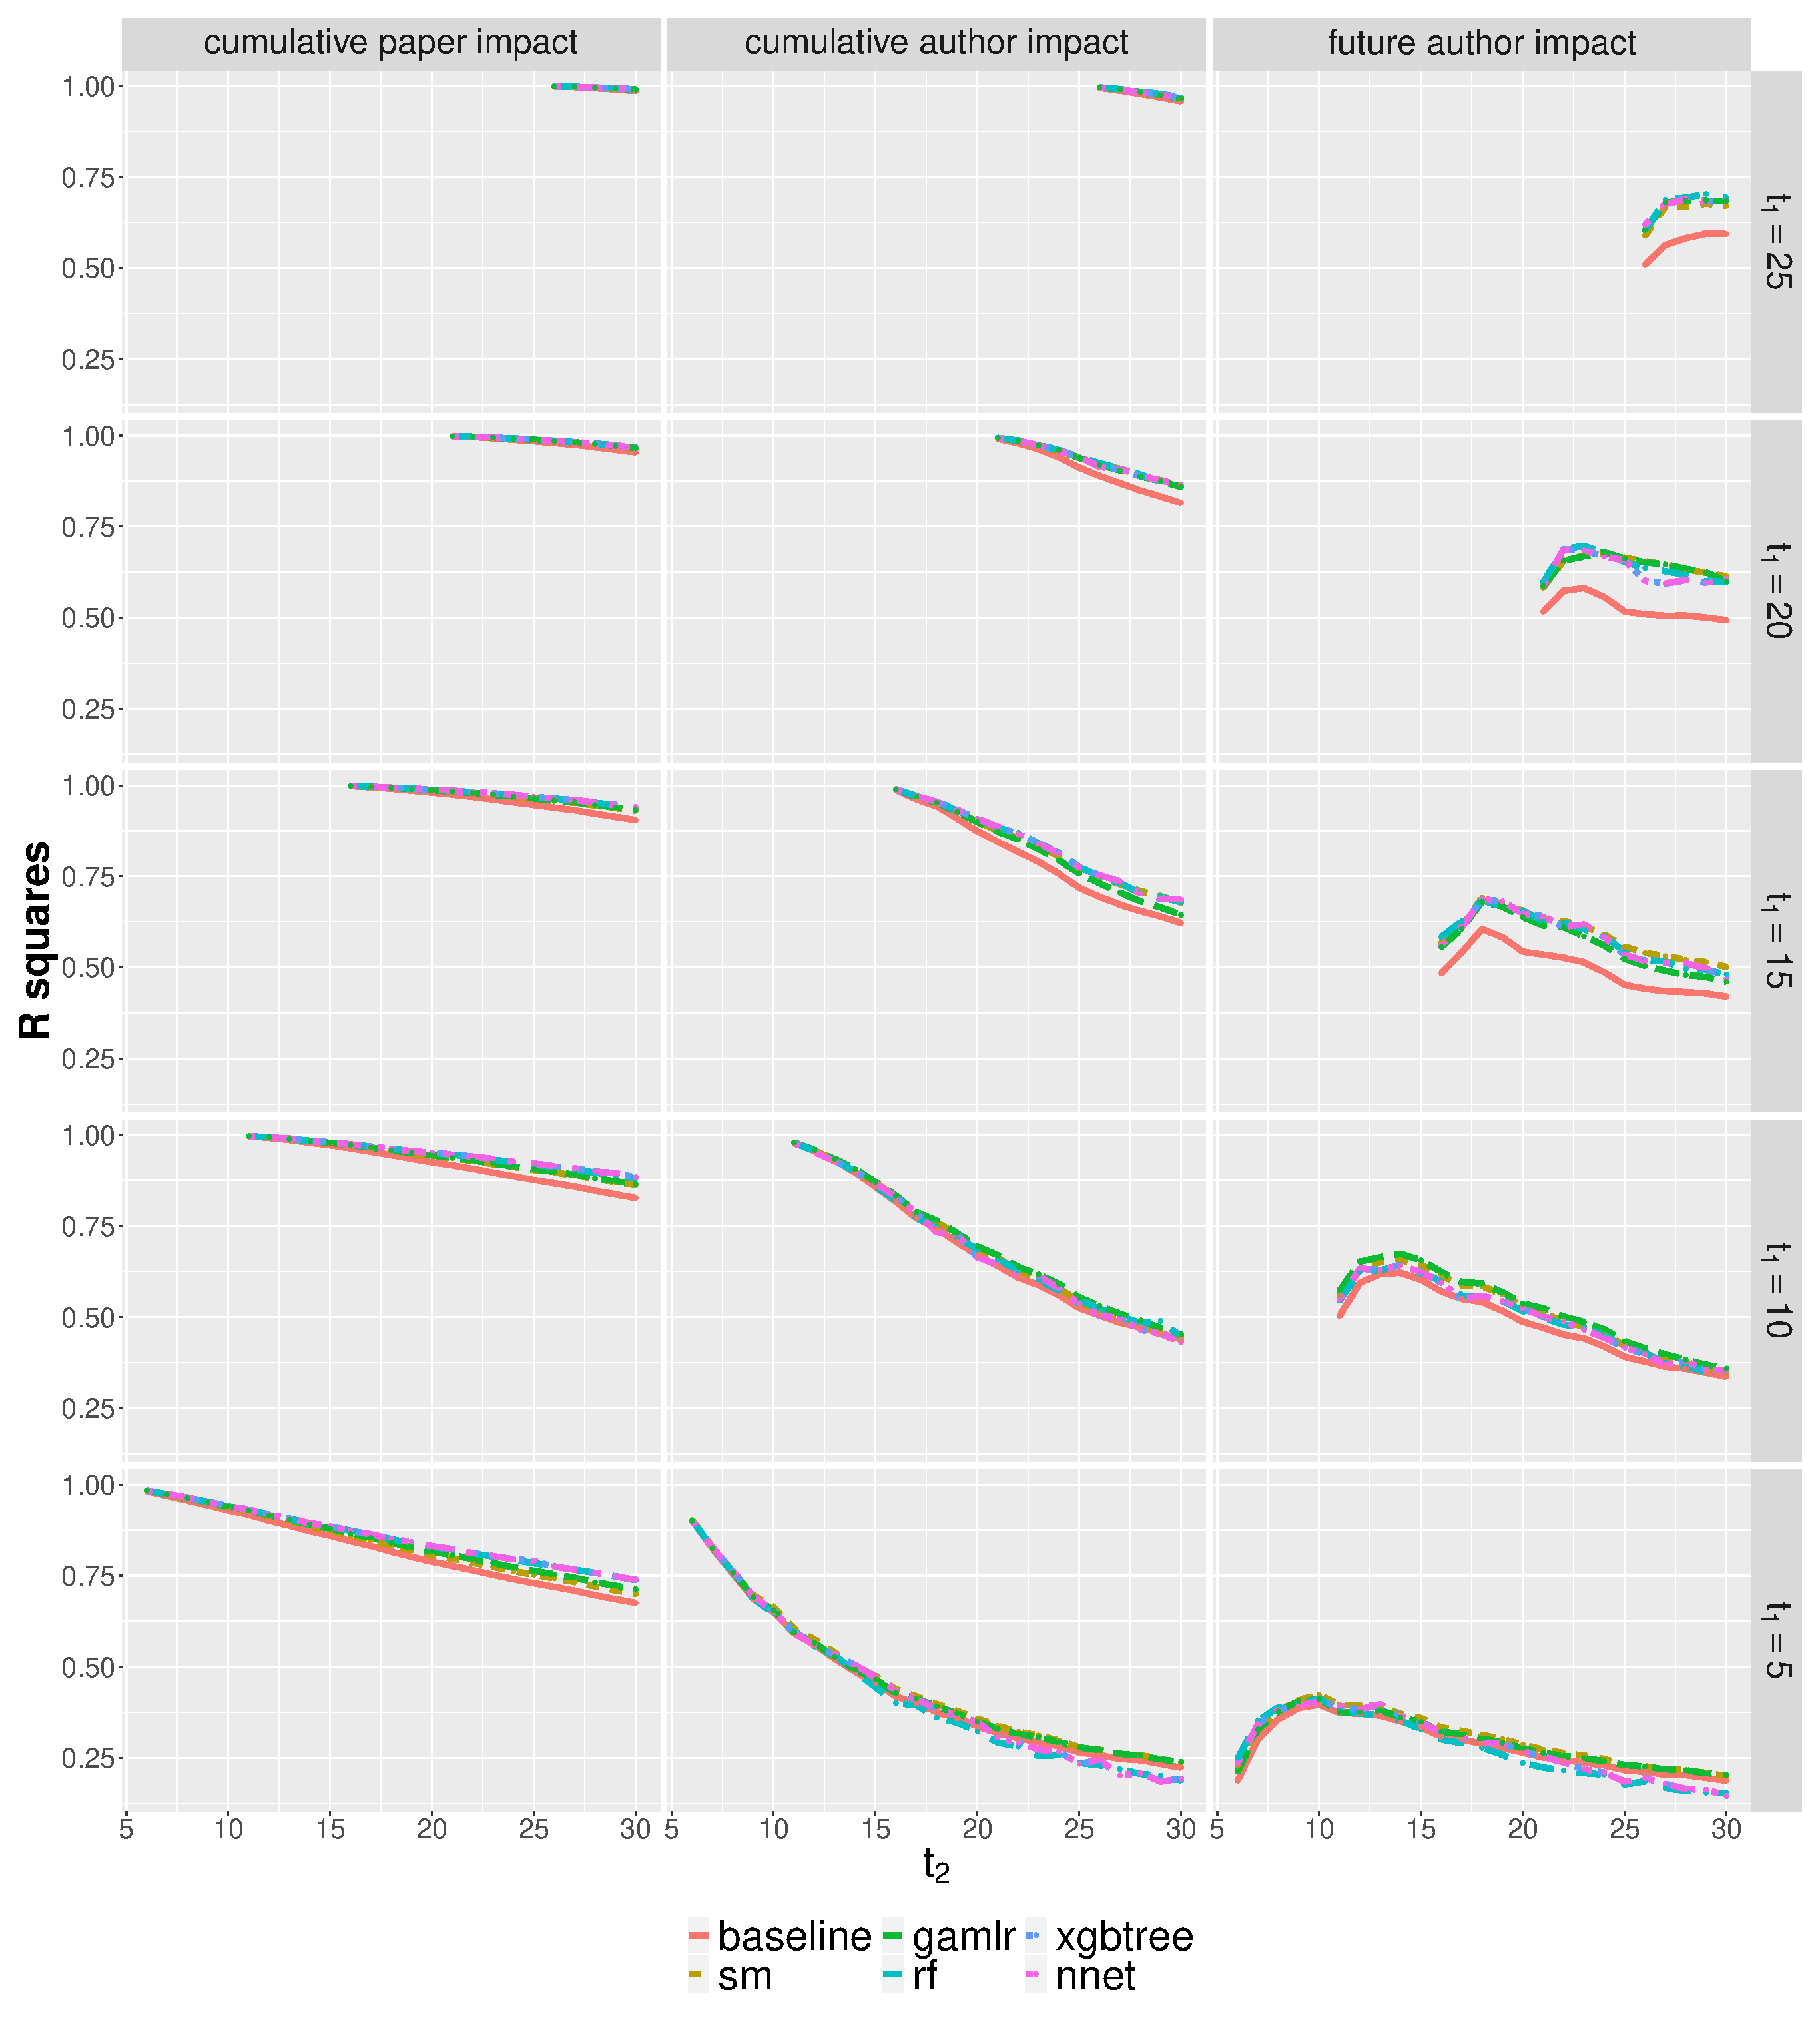
\includegraphics[width=\textwidth]{figures/pred_model/r2_diff.eps}
    \caption{Testing R squares of the predictive models. LASSO, ridge and elastic net are outperformed by Gamma LASSO, and hence are ignored for a better visualization.}
    \label{fig:pred_r2}
\end{figure}


\iffalse
\begin{figure}[ht!]
    \centering
        \begin{subfigure}[t]{0.8\textwidth}
        \centering
        \includegraphics[width=\textwidth]{figures/pred_model/pub/bio/importance.pdf}
        \caption{Top 5 features for predicting publication rp}
    \end{subfigure}%
    
    \begin{subfigure}[t]{0.8\textwidth}
        \centering
        \includegraphics[width=\textwidth]{figures/pred_model/aut/all/importance.pdf}
        \caption{Top 5 features for predicting author rp}
    \end{subfigure}

    \caption{Random permutation importance of features for predicting rank percentiles given by the random forest models. The top 5 features are selected based on the median of their importance values. }
    \label{fig:pred_model_importance}
\end{figure}
\fi
